% Capitolul 11: Ipoteza piețelor fractale și memoria lungă
% Statistica piețelor financiare -- Program de licență, Academia de Studii Economice din București
% GENERAT de latex/build_chapter11.py -- modificați generatorul, nu acest fișier.

\newcommand{\coursename}{Statistica piețelor financiare}
\def\sfmlang{ro}
% Preambul comun SFM -- Statistica piețelor financiare / Statistics of Financial Markets (Beamer, 16:9)
% Același design ca MFM. Înainte de % Preambul comun SFM -- Statistica piețelor financiare / Statistics of Financial Markets (Beamer, 16:9)
% Același design ca MFM. Înainte de % Preambul comun SFM -- Statistica piețelor financiare / Statistics of Financial Markets (Beamer, 16:9)
% Același design ca MFM. Înainte de \input{../../latex/preamble} se definește
%   \newcommand{\coursename}{Statistics of Financial Markets}      (EN)
%   \newcommand{\coursename}{Statistica piețelor financiare}       (RO)  și  \def\sfmlang{ro}
% Fișierele .tex se află în EN/Courses, EN/Seminars, RO/Cursuri, RO/Seminarii (două niveluri sub rădăcină).
% Deck-urile sînt generate de latex/build_chapterN.py / build_seminarN.py (vezi latex/sfm_build.py).

\documentclass[9pt, aspectratio=169, t]{beamer}
\providecommand{\coursename}{Statistics of Financial Markets}

% Ensure content fits on slides
\setbeamersize{text margin left=8mm, text margin right=8mm}

%=============================================================================
% THEME AND STYLE CONFIGURATION
%=============================================================================
\usetheme{default}
% Using default theme for clean header/footer control

% Color Palette (matching Redispatch PDF)
\definecolor{MainBlue}{RGB}{26, 58, 110}
\definecolor{AccentBlue}{RGB}{26, 58, 110}
\definecolor{IDAred}{RGB}{205, 0, 0}
\definecolor{DarkGray}{RGB}{51, 51, 51}
\definecolor{MediumGray}{RGB}{128, 128, 128}
\definecolor{LightGray}{RGB}{248, 248, 248}
\definecolor{VeryLightGray}{RGB}{235, 235, 235}
\definecolor{KeynoteGray}{RGB}{218, 218, 218}
\definecolor{SectionGray}{RGB}{120, 120, 120}
\definecolor{FooterGray}{RGB}{100, 100, 100}
\definecolor{Crimson}{RGB}{220, 53, 69}
\definecolor{Forest}{RGB}{46, 125, 50}
\definecolor{Amber}{RGB}{181, 133, 63}
\definecolor{Orange}{RGB}{230, 126, 34}
\definecolor{Purple}{RGB}{142, 68, 173}

% Gradient background (exact Keynote 315° gradient: white to RGB 218,218,218)
\setbeamertemplate{background}{%
    \begin{tikzpicture}[remember picture, overlay]
        \shade[shading=axis, shading angle=315,
        top color=white, bottom color=KeynoteGray]
        (current page.south west) rectangle (current page.north east);
    \end{tikzpicture}%
}
% Fallback solid color for compatibility
\setbeamercolor{background canvas}{bg=}

\setbeamercolor{palette primary}{bg=MainBlue, fg=white}
\setbeamercolor{palette secondary}{bg=MainBlue!85, fg=white}
\setbeamercolor{palette tertiary}{bg=MainBlue!70, fg=white}
\setbeamercolor{structure}{fg=MainBlue}
\setbeamercolor{title}{fg=IDAred}
\setbeamercolor{frametitle}{fg=IDAred, bg=}
\setbeamercolor{block title}{bg=MainBlue, fg=white}
\setbeamercolor{block body}{bg=VeryLightGray, fg=DarkGray}
\setbeamercolor{block title alerted}{bg=Crimson, fg=white}
\setbeamercolor{block body alerted}{bg=Crimson!8, fg=DarkGray}
\setbeamercolor{block title example}{bg=Forest, fg=white}
\setbeamercolor{block body example}{bg=Forest!8, fg=DarkGray}
\setbeamercolor{item}{fg=MainBlue}

% Footer colors (override Madrid theme blue)
\setbeamercolor{author in head/foot}{fg=FooterGray, bg=}
\setbeamercolor{title in head/foot}{fg=FooterGray, bg=}
\setbeamercolor{date in head/foot}{fg=FooterGray, bg=}
\setbeamercolor{section in head/foot}{fg=FooterGray, bg=}
\setbeamercolor{subsection in head/foot}{fg=FooterGray, bg=}

% Bullet styles (apply everywhere including blocks)
\setbeamertemplate{itemize item}{\color{MainBlue}$\boxdot$}
\setbeamertemplate{itemize subitem}{\color{MainBlue}$\blacktriangleright$}
\setbeamertemplate{itemize subsubitem}{\color{MainBlue}\tiny$\bullet$}
\setbeamertemplate{itemize/enumerate body begin}{\normalsize}
\setbeamertemplate{itemize/enumerate subbody begin}{\normalsize}

% Item spacing - compact style
\setlength{\leftmargini}{10pt}       % Level 1: minimal indent
\setlength{\leftmarginii}{10pt}      % Level 2: minimal additional indent
% Compact list spacing (zero extra space before/after lists in blocks)
\makeatletter
\def\@listi{\leftmargin\leftmargini \topsep 0pt \parsep 0pt \itemsep 0pt}
\def\@listii{\leftmargin\leftmarginii \topsep 0pt \parsep 0pt \itemsep 0pt}
\makeatother

\setbeamertemplate{navigation symbols}{}

%=============================================================================
% CUSTOM HEADLINE
%=============================================================================
\setbeamertemplate{headline}{%
    \vskip10pt%
    \hbox to \paperwidth{%
        \hskip0.5cm%
        {\small\color{FooterGray}\renewcommand{\hyperlink}[2]{##2}\insertsectionhead}%
        \hfill%
        \textcolor{FooterGray}{\small\insertframenumber}%
        \hskip0.5cm%
    }%
    \vskip4pt%
    {\color{FooterGray}\hrule height 0.4pt}%
}

%=============================================================================
% CUSTOM FOOTER
%=============================================================================
\usepackage{fontawesome5}

\setbeamertemplate{footline}{%
    {\color{FooterGray}\hrule height 0.4pt}%
    \vskip4pt%
    \hbox to \paperwidth{%
        \hskip0.5cm%
        \textcolor{FooterGray}{\small\coursename}%
        \hfill%
        \raisebox{-0.1em}{%
            \begin{tikzpicture}[x=0.08em, y=0.08em, line width=0.4pt]
                \draw[FooterGray] (0,3) -- (1,4) -- (2,3.5) -- (3,5) -- (4,4) -- (5,6) -- (6,5.5) -- (7,4) -- (8,5) -- (9,7) -- (10,6) -- (11,5) -- (12,6.5) -- (13,8) -- (14,7) -- (15,6) -- (16,7.5) -- (17,9) -- (18,8) -- (19,7) -- (20,8.5) -- (21,10) -- (22,9) -- (23,8) -- (24,9.5);
            \end{tikzpicture}%
        }%
        \hskip0.5cm%
    }%
    \vskip6pt%
}

%=============================================================================
% PACKAGES
%=============================================================================
\usepackage[utf8]{inputenc}
\DeclareUnicodeCharacter{03B1}{\ensuremath{\alpha}}
\usepackage[T1]{fontenc}
\usepackage{amsmath, amssymb, amsthm}
\usepackage{mathtools}
\usepackage{bm}
\usepackage{tikz}
\usetikzlibrary{arrows.meta, positioning, shapes, calc, decorations.pathreplacing, shadings}
\usepackage{booktabs}
\usepackage{multirow}
\usepackage{array}
\usepackage{graphicx}
\usepackage{hyperref}
\usepackage{colortbl}
\usepackage{listings}
\lstset{language=Python, basicstyle=\ttfamily\scriptsize, keywordstyle=\color{MainBlue}\bfseries,
  commentstyle=\color{Forest}, stringstyle=\color{Crimson}, breaklines=true,
  frame=none, backgroundcolor=\color{VeryLightGray}, xleftmargin=2mm}
\hypersetup{colorlinks=true, linkcolor=MainBlue, urlcolor=MainBlue}
\graphicspath{{../../logos/}{../../charts/}{../../photos/}}
\usepackage{xcolor}
\hfuzz=2pt  % Suppress tiny overfull warnings (<2pt)
\vfuzz=2pt  % Suppress tiny vertical overfull warnings (<2pt)

%=============================================================================
% QUANTLET COMMANDS
%   \quantlet{<displayed name>}{<url>}       (generic, compatible with the older SFM decks)
%   \sfmquantlet{Ch_05}{SFM_ch5_garch}       -> https://github.com/danpele/SFM/tree/main/Quantlets/Ch_05/SFM_ch5_garch
%   \qlurl{<folder>} is defined per chapter by the generator (Quantlets/Ch_NN/<folder>)
%=============================================================================
\newcommand{\sfmrepo}{https://github.com/danpele/SFM}
\newcommand{\sfmqlbase}{https://github.com/danpele/SFM/tree/main/Quantlets}
\newcommand{\quantlet}[2]{%
    \hfill\href{#2}{%
        \raisebox{-0.15em}{
\includegraphics[height=0.7em]{ql_logo.png}}%
        \textcolor{MainBlue}{\tiny\ #1}%
    }%
}
\newcommand{\sfmquantlet}[2]{\quantlet{\detokenize{#2}}{\sfmqlbase/#1/#2}}

%=============================================================================
% NOTEBOOKS (Google Colab)
%   \colaburl{notebooks/EN/chapter5_seminar_notebook.ipynb} -> the Colab link of a file in the SFM repo
%   \nb: the chapter notebook (each seminar deck redefines it with \renewcommand)
%=============================================================================
\newcommand{\colaburl}[1]{https://colab.research.google.com/github/danpele/SFM/blob/main/#1}
\newcommand{\nb}{https://colab.research.google.com/github/danpele/SFM/tree/main/notebooks/EN}
\newcommand{\nbname}{notebooks/EN}

%=============================================================================
% SLIDE HELPERS (used by the generators; the same as in MFM)
%=============================================================================
% local font size for list bodies (the preamble forces \normalsize)
\newcommand{\itemsize}[1]{\setbeamertemplate{itemize/enumerate body begin}{#1}\setbeamertemplate{itemize/enumerate subbody begin}{#1}}
\newcommand{\intitle}[1]{{\hypersetup{urlcolor=white}#1}}   % white links inside coloured title bars
\newcommand{\imgcap}[1]{{\scriptsize #1}\\[0.5mm]}          % caption under a photo
\newcommand{\imgcredit}[2]{{\tiny\color{FooterGray}\href{#1}{#2}}}   % image credit: source URL, author/licence
\newcommand{\aiprompt}[1]{{\ttfamily\color{MainBlue}#1}}     % a prompt to an AI assistant

%=============================================================================
% SEMINARS: student version by default; the instructor wrapper *_solutions.tex sets \solutionstrue
%=============================================================================
\makeatletter\@ifundefined{ifsolutions}{\expandafter\newif\csname ifsolutions\endcsname}{}\makeatother
\newcommand{\solonly}[1]{\ifsolutions #1\fi}
\newcommand{\propsub}{\ifsolutions\else\framesubtitle{\ifdefined\sfmlang Rezolvarea se discută la seminar\else Solution discussed in class\fi}\fi}

%=============================================================================
% APPENDIX AND CHAPTER LINKS (latex/appendix_links.py writes the calls; it also re-declares these
% macros before \begin{document}, so the decks compile with or without this preamble block)
%=============================================================================
\providecommand{\sfmapplink}[3]{\hypertarget{#2}{}\hyperlink{#1}{\beamergotobutton{#3}}}
\providecommand{\sfmappback}[2]{\begin{tikzpicture}[remember picture,overlay]\node[anchor=south east] at ([xshift=-3mm,yshift=7mm]current page.south east){\hyperlink{#1}{\beamerreturnbutton{#2}}};\end{tikzpicture}}
\providecommand{\sfmchlink}[2]{\href{#1}{#2}}
\providecommand{\sfmchlinkt}[2]{\href{#1}{\usebeamercolor[fg]{frametitle}#2}}

%=============================================================================
% QUANTINAR COMMAND: link către un curs Quantinar (subiecte avansate)
%=============================================================================
\newcommand{\quantinar}[2]{%
    \href{#2}{%
        \raisebox{-0.15em}{
\includegraphics[height=0.8em]{qr_logo.png}}%
        \textcolor{MainBlue}{\scriptsize\ #1}%
    }%
}

%=============================================================================
% CUSTOM TITLE PAGE
%=============================================================================
\defbeamertemplate*{title page}{hybrid}[1][]
{
    \vspace{0.2cm}
    % Logos row - top header (with clickable links)
    \begin{center}
        \href{https://www.ase.ro}{
\includegraphics[height=1.0cm]{ase_logo.png}}\hspace{0.3cm}%
        \href{https://theida.net}{
\includegraphics[height=1.0cm]{ida_logo.png}}\hspace{0.3cm}%
        \href{https://blockchain-research-center.com}{
\includegraphics[height=1.0cm]{brc_logo.png}}\hspace{0.3cm}%
        \href{https://www.ai4efin.ase.ro}{
\includegraphics[height=1.0cm]{ai4efin_logo.png}}\hspace{0.3cm}%
        \href{https://ipe.ro/new}{
\includegraphics[height=1.0cm]{acad_logo.png}}\hspace{0.3cm}%
        \href{https://www.digital-finance-msca.com}{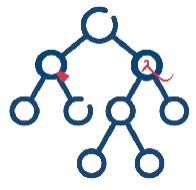
\includegraphics[height=1.0cm]{msca_logo.png}}%
    \end{center}

    \vspace{0.6cm}

    % Main title with Q logos on sides (with clickable links)
    \begin{center}
        \begin{minipage}{0.1\textwidth}
            \centering
            \href{https://quantlet.com}{
\includegraphics[height=1.1cm]{ql_logo.png}}
        \end{minipage}%
        \begin{minipage}{0.78\textwidth}
            \centering
            {\LARGE\bfseries\usebeamercolor[fg]{title}\inserttitle}

            \vspace{0.3cm}

            {\usebeamerfont{subtitle}\usebeamercolor[fg]{title}\insertsubtitle}
        \end{minipage}%
        \begin{minipage}{0.1\textwidth}
            \centering
            \href{https://quantinar.com}{
\includegraphics[height=1.1cm]{qr_logo.png}}
        \end{minipage}
    \end{center}

    \vspace{0.6cm}

    % Authors (left aligned)
    \hspace{0.5cm}{\usebeamerfont{author}\insertauthor}

    \vspace{0.3cm}

    % Institute/Affiliations (left aligned)
    \hspace{0.5cm}\begin{minipage}[t]{0.9\textwidth}
        \raggedright\small\insertinstitute
    \end{minipage}
}

%=============================================================================
% THEOREM ENVIRONMENTS
%=============================================================================
\theoremstyle{definition}
\setbeamertemplate{theorems}[numbered]
\ifdefined\sfmlang
\newtheorem{defn}{Definiție}
\newtheorem{thm}{Teoremă}
\newtheorem{prop}{Propoziție}
\newtheorem{rmk}{Observație}
\else
\newtheorem{defn}{Definition}
\newtheorem{thm}{Theorem}
\newtheorem{prop}{Proposition}
\newtheorem{rmk}{Remark}
\fi

%=============================================================================
% CENTRED MINIPAGE (no extra vertical space)
%=============================================================================
\newenvironment{cminipage}[1]{%
    \par\noindent\hfill\begin{minipage}{#1}\ignorespaces
}{%
    \end{minipage}\hfill\null\par
}

%=============================================================================
% CUSTOM COMMANDS
%=============================================================================
\newcommand{\E}{\mathbb{E}}
\newcommand{\Var}{\text{Var}}
\newcommand{\Cov}{\text{Cov}}
\newcommand{\Corr}{\text{Corr}}
\newcommand{\R}{\mathbb{R}}
\newcommand{\N}{\mathbb{N}}
\newcommand{\Z}{\mathbb{Z}}
\newcommand{\B}{\mathbf{B}}
\newcommand{\imark}{\textcolor{MainBlue}{\textbullet}}
\newcommand{\RMSE}{\text{RMSE}}
\newcommand{\MAE}{\text{MAE}}
\newcommand{\MAPE}{\text{MAPE}}

 se definește
%   \newcommand{\coursename}{Statistics of Financial Markets}      (EN)
%   \newcommand{\coursename}{Statistica piețelor financiare}       (RO)  și  \def\sfmlang{ro}
% Fișierele .tex se află în EN/Courses, EN/Seminars, RO/Cursuri, RO/Seminarii (două niveluri sub rădăcină).
% Deck-urile sînt generate de latex/build_chapterN.py / build_seminarN.py (vezi latex/sfm_build.py).

\documentclass[9pt, aspectratio=169, t]{beamer}
\providecommand{\coursename}{Statistics of Financial Markets}

% Ensure content fits on slides
\setbeamersize{text margin left=8mm, text margin right=8mm}

%=============================================================================
% THEME AND STYLE CONFIGURATION
%=============================================================================
\usetheme{default}
% Using default theme for clean header/footer control

% Color Palette (matching Redispatch PDF)
\definecolor{MainBlue}{RGB}{26, 58, 110}
\definecolor{AccentBlue}{RGB}{26, 58, 110}
\definecolor{IDAred}{RGB}{205, 0, 0}
\definecolor{DarkGray}{RGB}{51, 51, 51}
\definecolor{MediumGray}{RGB}{128, 128, 128}
\definecolor{LightGray}{RGB}{248, 248, 248}
\definecolor{VeryLightGray}{RGB}{235, 235, 235}
\definecolor{KeynoteGray}{RGB}{218, 218, 218}
\definecolor{SectionGray}{RGB}{120, 120, 120}
\definecolor{FooterGray}{RGB}{100, 100, 100}
\definecolor{Crimson}{RGB}{220, 53, 69}
\definecolor{Forest}{RGB}{46, 125, 50}
\definecolor{Amber}{RGB}{181, 133, 63}
\definecolor{Orange}{RGB}{230, 126, 34}
\definecolor{Purple}{RGB}{142, 68, 173}

% Gradient background (exact Keynote 315° gradient: white to RGB 218,218,218)
\setbeamertemplate{background}{%
    \begin{tikzpicture}[remember picture, overlay]
        \shade[shading=axis, shading angle=315,
        top color=white, bottom color=KeynoteGray]
        (current page.south west) rectangle (current page.north east);
    \end{tikzpicture}%
}
% Fallback solid color for compatibility
\setbeamercolor{background canvas}{bg=}

\setbeamercolor{palette primary}{bg=MainBlue, fg=white}
\setbeamercolor{palette secondary}{bg=MainBlue!85, fg=white}
\setbeamercolor{palette tertiary}{bg=MainBlue!70, fg=white}
\setbeamercolor{structure}{fg=MainBlue}
\setbeamercolor{title}{fg=IDAred}
\setbeamercolor{frametitle}{fg=IDAred, bg=}
\setbeamercolor{block title}{bg=MainBlue, fg=white}
\setbeamercolor{block body}{bg=VeryLightGray, fg=DarkGray}
\setbeamercolor{block title alerted}{bg=Crimson, fg=white}
\setbeamercolor{block body alerted}{bg=Crimson!8, fg=DarkGray}
\setbeamercolor{block title example}{bg=Forest, fg=white}
\setbeamercolor{block body example}{bg=Forest!8, fg=DarkGray}
\setbeamercolor{item}{fg=MainBlue}

% Footer colors (override Madrid theme blue)
\setbeamercolor{author in head/foot}{fg=FooterGray, bg=}
\setbeamercolor{title in head/foot}{fg=FooterGray, bg=}
\setbeamercolor{date in head/foot}{fg=FooterGray, bg=}
\setbeamercolor{section in head/foot}{fg=FooterGray, bg=}
\setbeamercolor{subsection in head/foot}{fg=FooterGray, bg=}

% Bullet styles (apply everywhere including blocks)
\setbeamertemplate{itemize item}{\color{MainBlue}$\boxdot$}
\setbeamertemplate{itemize subitem}{\color{MainBlue}$\blacktriangleright$}
\setbeamertemplate{itemize subsubitem}{\color{MainBlue}\tiny$\bullet$}
\setbeamertemplate{itemize/enumerate body begin}{\normalsize}
\setbeamertemplate{itemize/enumerate subbody begin}{\normalsize}

% Item spacing - compact style
\setlength{\leftmargini}{10pt}       % Level 1: minimal indent
\setlength{\leftmarginii}{10pt}      % Level 2: minimal additional indent
% Compact list spacing (zero extra space before/after lists in blocks)
\makeatletter
\def\@listi{\leftmargin\leftmargini \topsep 0pt \parsep 0pt \itemsep 0pt}
\def\@listii{\leftmargin\leftmarginii \topsep 0pt \parsep 0pt \itemsep 0pt}
\makeatother

\setbeamertemplate{navigation symbols}{}

%=============================================================================
% CUSTOM HEADLINE
%=============================================================================
\setbeamertemplate{headline}{%
    \vskip10pt%
    \hbox to \paperwidth{%
        \hskip0.5cm%
        {\small\color{FooterGray}\renewcommand{\hyperlink}[2]{##2}\insertsectionhead}%
        \hfill%
        \textcolor{FooterGray}{\small\insertframenumber}%
        \hskip0.5cm%
    }%
    \vskip4pt%
    {\color{FooterGray}\hrule height 0.4pt}%
}

%=============================================================================
% CUSTOM FOOTER
%=============================================================================
\usepackage{fontawesome5}

\setbeamertemplate{footline}{%
    {\color{FooterGray}\hrule height 0.4pt}%
    \vskip4pt%
    \hbox to \paperwidth{%
        \hskip0.5cm%
        \textcolor{FooterGray}{\small\coursename}%
        \hfill%
        \raisebox{-0.1em}{%
            \begin{tikzpicture}[x=0.08em, y=0.08em, line width=0.4pt]
                \draw[FooterGray] (0,3) -- (1,4) -- (2,3.5) -- (3,5) -- (4,4) -- (5,6) -- (6,5.5) -- (7,4) -- (8,5) -- (9,7) -- (10,6) -- (11,5) -- (12,6.5) -- (13,8) -- (14,7) -- (15,6) -- (16,7.5) -- (17,9) -- (18,8) -- (19,7) -- (20,8.5) -- (21,10) -- (22,9) -- (23,8) -- (24,9.5);
            \end{tikzpicture}%
        }%
        \hskip0.5cm%
    }%
    \vskip6pt%
}

%=============================================================================
% PACKAGES
%=============================================================================
\usepackage[utf8]{inputenc}
\DeclareUnicodeCharacter{03B1}{\ensuremath{\alpha}}
\usepackage[T1]{fontenc}
\usepackage{amsmath, amssymb, amsthm}
\usepackage{mathtools}
\usepackage{bm}
\usepackage{tikz}
\usetikzlibrary{arrows.meta, positioning, shapes, calc, decorations.pathreplacing, shadings}
\usepackage{booktabs}
\usepackage{multirow}
\usepackage{array}
\usepackage{graphicx}
\usepackage{hyperref}
\usepackage{colortbl}
\usepackage{listings}
\lstset{language=Python, basicstyle=\ttfamily\scriptsize, keywordstyle=\color{MainBlue}\bfseries,
  commentstyle=\color{Forest}, stringstyle=\color{Crimson}, breaklines=true,
  frame=none, backgroundcolor=\color{VeryLightGray}, xleftmargin=2mm}
\hypersetup{colorlinks=true, linkcolor=MainBlue, urlcolor=MainBlue}
\graphicspath{{../../logos/}{../../charts/}{../../photos/}}
\usepackage{xcolor}
\hfuzz=2pt  % Suppress tiny overfull warnings (<2pt)
\vfuzz=2pt  % Suppress tiny vertical overfull warnings (<2pt)

%=============================================================================
% QUANTLET COMMANDS
%   \quantlet{<displayed name>}{<url>}       (generic, compatible with the older SFM decks)
%   \sfmquantlet{Ch_05}{SFM_ch5_garch}       -> https://github.com/danpele/SFM/tree/main/Quantlets/Ch_05/SFM_ch5_garch
%   \qlurl{<folder>} is defined per chapter by the generator (Quantlets/Ch_NN/<folder>)
%=============================================================================
\newcommand{\sfmrepo}{https://github.com/danpele/SFM}
\newcommand{\sfmqlbase}{https://github.com/danpele/SFM/tree/main/Quantlets}
\newcommand{\quantlet}[2]{%
    \hfill\href{#2}{%
        \raisebox{-0.15em}{
\includegraphics[height=0.7em]{ql_logo.png}}%
        \textcolor{MainBlue}{\tiny\ #1}%
    }%
}
\newcommand{\sfmquantlet}[2]{\quantlet{\detokenize{#2}}{\sfmqlbase/#1/#2}}

%=============================================================================
% NOTEBOOKS (Google Colab)
%   \colaburl{notebooks/EN/chapter5_seminar_notebook.ipynb} -> the Colab link of a file in the SFM repo
%   \nb: the chapter notebook (each seminar deck redefines it with \renewcommand)
%=============================================================================
\newcommand{\colaburl}[1]{https://colab.research.google.com/github/danpele/SFM/blob/main/#1}
\newcommand{\nb}{https://colab.research.google.com/github/danpele/SFM/tree/main/notebooks/EN}
\newcommand{\nbname}{notebooks/EN}

%=============================================================================
% SLIDE HELPERS (used by the generators; the same as in MFM)
%=============================================================================
% local font size for list bodies (the preamble forces \normalsize)
\newcommand{\itemsize}[1]{\setbeamertemplate{itemize/enumerate body begin}{#1}\setbeamertemplate{itemize/enumerate subbody begin}{#1}}
\newcommand{\intitle}[1]{{\hypersetup{urlcolor=white}#1}}   % white links inside coloured title bars
\newcommand{\imgcap}[1]{{\scriptsize #1}\\[0.5mm]}          % caption under a photo
\newcommand{\imgcredit}[2]{{\tiny\color{FooterGray}\href{#1}{#2}}}   % image credit: source URL, author/licence
\newcommand{\aiprompt}[1]{{\ttfamily\color{MainBlue}#1}}     % a prompt to an AI assistant

%=============================================================================
% SEMINARS: student version by default; the instructor wrapper *_solutions.tex sets \solutionstrue
%=============================================================================
\makeatletter\@ifundefined{ifsolutions}{\expandafter\newif\csname ifsolutions\endcsname}{}\makeatother
\newcommand{\solonly}[1]{\ifsolutions #1\fi}
\newcommand{\propsub}{\ifsolutions\else\framesubtitle{\ifdefined\sfmlang Rezolvarea se discută la seminar\else Solution discussed in class\fi}\fi}

%=============================================================================
% APPENDIX AND CHAPTER LINKS (latex/appendix_links.py writes the calls; it also re-declares these
% macros before \begin{document}, so the decks compile with or without this preamble block)
%=============================================================================
\providecommand{\sfmapplink}[3]{\hypertarget{#2}{}\hyperlink{#1}{\beamergotobutton{#3}}}
\providecommand{\sfmappback}[2]{\begin{tikzpicture}[remember picture,overlay]\node[anchor=south east] at ([xshift=-3mm,yshift=7mm]current page.south east){\hyperlink{#1}{\beamerreturnbutton{#2}}};\end{tikzpicture}}
\providecommand{\sfmchlink}[2]{\href{#1}{#2}}
\providecommand{\sfmchlinkt}[2]{\href{#1}{\usebeamercolor[fg]{frametitle}#2}}

%=============================================================================
% QUANTINAR COMMAND: link către un curs Quantinar (subiecte avansate)
%=============================================================================
\newcommand{\quantinar}[2]{%
    \href{#2}{%
        \raisebox{-0.15em}{
\includegraphics[height=0.8em]{qr_logo.png}}%
        \textcolor{MainBlue}{\scriptsize\ #1}%
    }%
}

%=============================================================================
% CUSTOM TITLE PAGE
%=============================================================================
\defbeamertemplate*{title page}{hybrid}[1][]
{
    \vspace{0.2cm}
    % Logos row - top header (with clickable links)
    \begin{center}
        \href{https://www.ase.ro}{
\includegraphics[height=1.0cm]{ase_logo.png}}\hspace{0.3cm}%
        \href{https://theida.net}{
\includegraphics[height=1.0cm]{ida_logo.png}}\hspace{0.3cm}%
        \href{https://blockchain-research-center.com}{
\includegraphics[height=1.0cm]{brc_logo.png}}\hspace{0.3cm}%
        \href{https://www.ai4efin.ase.ro}{
\includegraphics[height=1.0cm]{ai4efin_logo.png}}\hspace{0.3cm}%
        \href{https://ipe.ro/new}{
\includegraphics[height=1.0cm]{acad_logo.png}}\hspace{0.3cm}%
        \href{https://www.digital-finance-msca.com}{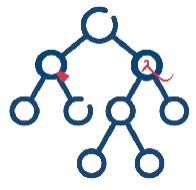
\includegraphics[height=1.0cm]{msca_logo.png}}%
    \end{center}

    \vspace{0.6cm}

    % Main title with Q logos on sides (with clickable links)
    \begin{center}
        \begin{minipage}{0.1\textwidth}
            \centering
            \href{https://quantlet.com}{
\includegraphics[height=1.1cm]{ql_logo.png}}
        \end{minipage}%
        \begin{minipage}{0.78\textwidth}
            \centering
            {\LARGE\bfseries\usebeamercolor[fg]{title}\inserttitle}

            \vspace{0.3cm}

            {\usebeamerfont{subtitle}\usebeamercolor[fg]{title}\insertsubtitle}
        \end{minipage}%
        \begin{minipage}{0.1\textwidth}
            \centering
            \href{https://quantinar.com}{
\includegraphics[height=1.1cm]{qr_logo.png}}
        \end{minipage}
    \end{center}

    \vspace{0.6cm}

    % Authors (left aligned)
    \hspace{0.5cm}{\usebeamerfont{author}\insertauthor}

    \vspace{0.3cm}

    % Institute/Affiliations (left aligned)
    \hspace{0.5cm}\begin{minipage}[t]{0.9\textwidth}
        \raggedright\small\insertinstitute
    \end{minipage}
}

%=============================================================================
% THEOREM ENVIRONMENTS
%=============================================================================
\theoremstyle{definition}
\setbeamertemplate{theorems}[numbered]
\ifdefined\sfmlang
\newtheorem{defn}{Definiție}
\newtheorem{thm}{Teoremă}
\newtheorem{prop}{Propoziție}
\newtheorem{rmk}{Observație}
\else
\newtheorem{defn}{Definition}
\newtheorem{thm}{Theorem}
\newtheorem{prop}{Proposition}
\newtheorem{rmk}{Remark}
\fi

%=============================================================================
% CENTRED MINIPAGE (no extra vertical space)
%=============================================================================
\newenvironment{cminipage}[1]{%
    \par\noindent\hfill\begin{minipage}{#1}\ignorespaces
}{%
    \end{minipage}\hfill\null\par
}

%=============================================================================
% CUSTOM COMMANDS
%=============================================================================
\newcommand{\E}{\mathbb{E}}
\newcommand{\Var}{\text{Var}}
\newcommand{\Cov}{\text{Cov}}
\newcommand{\Corr}{\text{Corr}}
\newcommand{\R}{\mathbb{R}}
\newcommand{\N}{\mathbb{N}}
\newcommand{\Z}{\mathbb{Z}}
\newcommand{\B}{\mathbf{B}}
\newcommand{\imark}{\textcolor{MainBlue}{\textbullet}}
\newcommand{\RMSE}{\text{RMSE}}
\newcommand{\MAE}{\text{MAE}}
\newcommand{\MAPE}{\text{MAPE}}

 se definește
%   \newcommand{\coursename}{Statistics of Financial Markets}      (EN)
%   \newcommand{\coursename}{Statistica piețelor financiare}       (RO)  și  \def\sfmlang{ro}
% Fișierele .tex se află în EN/Courses, EN/Seminars, RO/Cursuri, RO/Seminarii (două niveluri sub rădăcină).
% Deck-urile sînt generate de latex/build_chapterN.py / build_seminarN.py (vezi latex/sfm_build.py).

\documentclass[9pt, aspectratio=169, t]{beamer}
\providecommand{\coursename}{Statistics of Financial Markets}

% Ensure content fits on slides
\setbeamersize{text margin left=8mm, text margin right=8mm}

%=============================================================================
% THEME AND STYLE CONFIGURATION
%=============================================================================
\usetheme{default}
% Using default theme for clean header/footer control

% Color Palette (matching Redispatch PDF)
\definecolor{MainBlue}{RGB}{26, 58, 110}
\definecolor{AccentBlue}{RGB}{26, 58, 110}
\definecolor{IDAred}{RGB}{205, 0, 0}
\definecolor{DarkGray}{RGB}{51, 51, 51}
\definecolor{MediumGray}{RGB}{128, 128, 128}
\definecolor{LightGray}{RGB}{248, 248, 248}
\definecolor{VeryLightGray}{RGB}{235, 235, 235}
\definecolor{KeynoteGray}{RGB}{218, 218, 218}
\definecolor{SectionGray}{RGB}{120, 120, 120}
\definecolor{FooterGray}{RGB}{100, 100, 100}
\definecolor{Crimson}{RGB}{220, 53, 69}
\definecolor{Forest}{RGB}{46, 125, 50}
\definecolor{Amber}{RGB}{181, 133, 63}
\definecolor{Orange}{RGB}{230, 126, 34}
\definecolor{Purple}{RGB}{142, 68, 173}

% Gradient background (exact Keynote 315° gradient: white to RGB 218,218,218)
\setbeamertemplate{background}{%
    \begin{tikzpicture}[remember picture, overlay]
        \shade[shading=axis, shading angle=315,
        top color=white, bottom color=KeynoteGray]
        (current page.south west) rectangle (current page.north east);
    \end{tikzpicture}%
}
% Fallback solid color for compatibility
\setbeamercolor{background canvas}{bg=}

\setbeamercolor{palette primary}{bg=MainBlue, fg=white}
\setbeamercolor{palette secondary}{bg=MainBlue!85, fg=white}
\setbeamercolor{palette tertiary}{bg=MainBlue!70, fg=white}
\setbeamercolor{structure}{fg=MainBlue}
\setbeamercolor{title}{fg=IDAred}
\setbeamercolor{frametitle}{fg=IDAred, bg=}
\setbeamercolor{block title}{bg=MainBlue, fg=white}
\setbeamercolor{block body}{bg=VeryLightGray, fg=DarkGray}
\setbeamercolor{block title alerted}{bg=Crimson, fg=white}
\setbeamercolor{block body alerted}{bg=Crimson!8, fg=DarkGray}
\setbeamercolor{block title example}{bg=Forest, fg=white}
\setbeamercolor{block body example}{bg=Forest!8, fg=DarkGray}
\setbeamercolor{item}{fg=MainBlue}

% Footer colors (override Madrid theme blue)
\setbeamercolor{author in head/foot}{fg=FooterGray, bg=}
\setbeamercolor{title in head/foot}{fg=FooterGray, bg=}
\setbeamercolor{date in head/foot}{fg=FooterGray, bg=}
\setbeamercolor{section in head/foot}{fg=FooterGray, bg=}
\setbeamercolor{subsection in head/foot}{fg=FooterGray, bg=}

% Bullet styles (apply everywhere including blocks)
\setbeamertemplate{itemize item}{\color{MainBlue}$\boxdot$}
\setbeamertemplate{itemize subitem}{\color{MainBlue}$\blacktriangleright$}
\setbeamertemplate{itemize subsubitem}{\color{MainBlue}\tiny$\bullet$}
\setbeamertemplate{itemize/enumerate body begin}{\normalsize}
\setbeamertemplate{itemize/enumerate subbody begin}{\normalsize}

% Item spacing - compact style
\setlength{\leftmargini}{10pt}       % Level 1: minimal indent
\setlength{\leftmarginii}{10pt}      % Level 2: minimal additional indent
% Compact list spacing (zero extra space before/after lists in blocks)
\makeatletter
\def\@listi{\leftmargin\leftmargini \topsep 0pt \parsep 0pt \itemsep 0pt}
\def\@listii{\leftmargin\leftmarginii \topsep 0pt \parsep 0pt \itemsep 0pt}
\makeatother

\setbeamertemplate{navigation symbols}{}

%=============================================================================
% CUSTOM HEADLINE
%=============================================================================
\setbeamertemplate{headline}{%
    \vskip10pt%
    \hbox to \paperwidth{%
        \hskip0.5cm%
        {\small\color{FooterGray}\renewcommand{\hyperlink}[2]{##2}\insertsectionhead}%
        \hfill%
        \textcolor{FooterGray}{\small\insertframenumber}%
        \hskip0.5cm%
    }%
    \vskip4pt%
    {\color{FooterGray}\hrule height 0.4pt}%
}

%=============================================================================
% CUSTOM FOOTER
%=============================================================================
\usepackage{fontawesome5}

\setbeamertemplate{footline}{%
    {\color{FooterGray}\hrule height 0.4pt}%
    \vskip4pt%
    \hbox to \paperwidth{%
        \hskip0.5cm%
        \textcolor{FooterGray}{\small\coursename}%
        \hfill%
        \raisebox{-0.1em}{%
            \begin{tikzpicture}[x=0.08em, y=0.08em, line width=0.4pt]
                \draw[FooterGray] (0,3) -- (1,4) -- (2,3.5) -- (3,5) -- (4,4) -- (5,6) -- (6,5.5) -- (7,4) -- (8,5) -- (9,7) -- (10,6) -- (11,5) -- (12,6.5) -- (13,8) -- (14,7) -- (15,6) -- (16,7.5) -- (17,9) -- (18,8) -- (19,7) -- (20,8.5) -- (21,10) -- (22,9) -- (23,8) -- (24,9.5);
            \end{tikzpicture}%
        }%
        \hskip0.5cm%
    }%
    \vskip6pt%
}

%=============================================================================
% PACKAGES
%=============================================================================
\usepackage[utf8]{inputenc}
\DeclareUnicodeCharacter{03B1}{\ensuremath{\alpha}}
\usepackage[T1]{fontenc}
\usepackage{amsmath, amssymb, amsthm}
\usepackage{mathtools}
\usepackage{bm}
\usepackage{tikz}
\usetikzlibrary{arrows.meta, positioning, shapes, calc, decorations.pathreplacing, shadings}
\usepackage{booktabs}
\usepackage{multirow}
\usepackage{array}
\usepackage{graphicx}
\usepackage{hyperref}
\usepackage{colortbl}
\usepackage{listings}
\lstset{language=Python, basicstyle=\ttfamily\scriptsize, keywordstyle=\color{MainBlue}\bfseries,
  commentstyle=\color{Forest}, stringstyle=\color{Crimson}, breaklines=true,
  frame=none, backgroundcolor=\color{VeryLightGray}, xleftmargin=2mm}
\hypersetup{colorlinks=true, linkcolor=MainBlue, urlcolor=MainBlue}
\graphicspath{{../../logos/}{../../charts/}{../../photos/}}
\usepackage{xcolor}
\hfuzz=2pt  % Suppress tiny overfull warnings (<2pt)
\vfuzz=2pt  % Suppress tiny vertical overfull warnings (<2pt)

%=============================================================================
% QUANTLET COMMANDS
%   \quantlet{<displayed name>}{<url>}       (generic, compatible with the older SFM decks)
%   \sfmquantlet{Ch_05}{SFM_ch5_garch}       -> https://github.com/danpele/SFM/tree/main/Quantlets/Ch_05/SFM_ch5_garch
%   \qlurl{<folder>} is defined per chapter by the generator (Quantlets/Ch_NN/<folder>)
%=============================================================================
\newcommand{\sfmrepo}{https://github.com/danpele/SFM}
\newcommand{\sfmqlbase}{https://github.com/danpele/SFM/tree/main/Quantlets}
\newcommand{\quantlet}[2]{%
    \hfill\href{#2}{%
        \raisebox{-0.15em}{
\includegraphics[height=0.7em]{ql_logo.png}}%
        \textcolor{MainBlue}{\tiny\ #1}%
    }%
}
\newcommand{\sfmquantlet}[2]{\quantlet{\detokenize{#2}}{\sfmqlbase/#1/#2}}

%=============================================================================
% NOTEBOOKS (Google Colab)
%   \colaburl{notebooks/EN/chapter5_seminar_notebook.ipynb} -> the Colab link of a file in the SFM repo
%   \nb: the chapter notebook (each seminar deck redefines it with \renewcommand)
%=============================================================================
\newcommand{\colaburl}[1]{https://colab.research.google.com/github/danpele/SFM/blob/main/#1}
\newcommand{\nb}{https://colab.research.google.com/github/danpele/SFM/tree/main/notebooks/EN}
\newcommand{\nbname}{notebooks/EN}

%=============================================================================
% SLIDE HELPERS (used by the generators; the same as in MFM)
%=============================================================================
% local font size for list bodies (the preamble forces \normalsize)
\newcommand{\itemsize}[1]{\setbeamertemplate{itemize/enumerate body begin}{#1}\setbeamertemplate{itemize/enumerate subbody begin}{#1}}
\newcommand{\intitle}[1]{{\hypersetup{urlcolor=white}#1}}   % white links inside coloured title bars
\newcommand{\imgcap}[1]{{\scriptsize #1}\\[0.5mm]}          % caption under a photo
\newcommand{\imgcredit}[2]{{\tiny\color{FooterGray}\href{#1}{#2}}}   % image credit: source URL, author/licence
\newcommand{\aiprompt}[1]{{\ttfamily\color{MainBlue}#1}}     % a prompt to an AI assistant

%=============================================================================
% SEMINARS: student version by default; the instructor wrapper *_solutions.tex sets \solutionstrue
%=============================================================================
\makeatletter\@ifundefined{ifsolutions}{\expandafter\newif\csname ifsolutions\endcsname}{}\makeatother
\newcommand{\solonly}[1]{\ifsolutions #1\fi}
\newcommand{\propsub}{\ifsolutions\else\framesubtitle{\ifdefined\sfmlang Rezolvarea se discută la seminar\else Solution discussed in class\fi}\fi}

%=============================================================================
% APPENDIX AND CHAPTER LINKS (latex/appendix_links.py writes the calls; it also re-declares these
% macros before \begin{document}, so the decks compile with or without this preamble block)
%=============================================================================
\providecommand{\sfmapplink}[3]{\hypertarget{#2}{}\hyperlink{#1}{\beamergotobutton{#3}}}
\providecommand{\sfmappback}[2]{\begin{tikzpicture}[remember picture,overlay]\node[anchor=south east] at ([xshift=-3mm,yshift=7mm]current page.south east){\hyperlink{#1}{\beamerreturnbutton{#2}}};\end{tikzpicture}}
\providecommand{\sfmchlink}[2]{\href{#1}{#2}}
\providecommand{\sfmchlinkt}[2]{\href{#1}{\usebeamercolor[fg]{frametitle}#2}}

%=============================================================================
% QUANTINAR COMMAND: link către un curs Quantinar (subiecte avansate)
%=============================================================================
\newcommand{\quantinar}[2]{%
    \href{#2}{%
        \raisebox{-0.15em}{
\includegraphics[height=0.8em]{qr_logo.png}}%
        \textcolor{MainBlue}{\scriptsize\ #1}%
    }%
}

%=============================================================================
% CUSTOM TITLE PAGE
%=============================================================================
\defbeamertemplate*{title page}{hybrid}[1][]
{
    \vspace{0.2cm}
    % Logos row - top header (with clickable links)
    \begin{center}
        \href{https://www.ase.ro}{
\includegraphics[height=1.0cm]{ase_logo.png}}\hspace{0.3cm}%
        \href{https://theida.net}{
\includegraphics[height=1.0cm]{ida_logo.png}}\hspace{0.3cm}%
        \href{https://blockchain-research-center.com}{
\includegraphics[height=1.0cm]{brc_logo.png}}\hspace{0.3cm}%
        \href{https://www.ai4efin.ase.ro}{
\includegraphics[height=1.0cm]{ai4efin_logo.png}}\hspace{0.3cm}%
        \href{https://ipe.ro/new}{
\includegraphics[height=1.0cm]{acad_logo.png}}\hspace{0.3cm}%
        \href{https://www.digital-finance-msca.com}{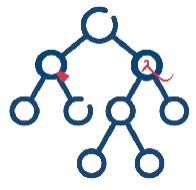
\includegraphics[height=1.0cm]{msca_logo.png}}%
    \end{center}

    \vspace{0.6cm}

    % Main title with Q logos on sides (with clickable links)
    \begin{center}
        \begin{minipage}{0.1\textwidth}
            \centering
            \href{https://quantlet.com}{
\includegraphics[height=1.1cm]{ql_logo.png}}
        \end{minipage}%
        \begin{minipage}{0.78\textwidth}
            \centering
            {\LARGE\bfseries\usebeamercolor[fg]{title}\inserttitle}

            \vspace{0.3cm}

            {\usebeamerfont{subtitle}\usebeamercolor[fg]{title}\insertsubtitle}
        \end{minipage}%
        \begin{minipage}{0.1\textwidth}
            \centering
            \href{https://quantinar.com}{
\includegraphics[height=1.1cm]{qr_logo.png}}
        \end{minipage}
    \end{center}

    \vspace{0.6cm}

    % Authors (left aligned)
    \hspace{0.5cm}{\usebeamerfont{author}\insertauthor}

    \vspace{0.3cm}

    % Institute/Affiliations (left aligned)
    \hspace{0.5cm}\begin{minipage}[t]{0.9\textwidth}
        \raggedright\small\insertinstitute
    \end{minipage}
}

%=============================================================================
% THEOREM ENVIRONMENTS
%=============================================================================
\theoremstyle{definition}
\setbeamertemplate{theorems}[numbered]
\ifdefined\sfmlang
\newtheorem{defn}{Definiție}
\newtheorem{thm}{Teoremă}
\newtheorem{prop}{Propoziție}
\newtheorem{rmk}{Observație}
\else
\newtheorem{defn}{Definition}
\newtheorem{thm}{Theorem}
\newtheorem{prop}{Proposition}
\newtheorem{rmk}{Remark}
\fi

%=============================================================================
% CENTRED MINIPAGE (no extra vertical space)
%=============================================================================
\newenvironment{cminipage}[1]{%
    \par\noindent\hfill\begin{minipage}{#1}\ignorespaces
}{%
    \end{minipage}\hfill\null\par
}

%=============================================================================
% CUSTOM COMMANDS
%=============================================================================
\newcommand{\E}{\mathbb{E}}
\newcommand{\Var}{\text{Var}}
\newcommand{\Cov}{\text{Cov}}
\newcommand{\Corr}{\text{Corr}}
\newcommand{\R}{\mathbb{R}}
\newcommand{\N}{\mathbb{N}}
\newcommand{\Z}{\mathbb{Z}}
\newcommand{\B}{\mathbf{B}}
\newcommand{\imark}{\textcolor{MainBlue}{\textbullet}}
\newcommand{\RMSE}{\text{RMSE}}
\newcommand{\MAE}{\text{MAE}}
\newcommand{\MAPE}{\text{MAPE}}



\newcommand{\qlurl}[1]{https://github.com/danpele/SFM/tree/main/Quantlets/Ch_11/#1}

% Clickable citations (DOIs verified via Crossref)

\newcommand{\refPeters}{\href{https://www.wiley.com/en-us/Fractal+Market+Analysis\%3A+Applying+Chaos+Theory+to+Investment+and+Economics-p-9780471585244}{Peters (1994)}}
\newcommand{\refFama}{\href{https://doi.org/10.2307/2325486}{Fama (1970)}}
\newcommand{\refLoAMH}{\href{https://doi.org/10.3905/jpm.2004.442611}{Lo (2004)}}
\newcommand{\refMan}{\href{https://doi.org/10.1086/294632}{Mandelbrot (1963)}}
\newcommand{\refCoast}{\href{https://doi.org/10.1126/science.156.3775.636}{Mandelbrot (1967)}}
\newcommand{\refMVN}{\href{https://doi.org/10.1137/1010093}{Mandelbrot \& Van Ness (1968)}}
\newcommand{\refNoah}{\href{https://doi.org/10.1029/WR004i005p00909}{Mandelbrot \& Wallis (1968)}}
\newcommand{\refMW}{\href{https://doi.org/10.1029/WR005i005p00967}{Mandelbrot \& Wallis (1969)}}
\newcommand{\refHurst}{\href{https://doi.org/10.1061/TACEAT.0006518}{Hurst (1951)}}
\newcommand{\refAL}{\href{https://doi.org/10.1093/biomet/63.1.111}{Anis \& Lloyd (1976)}}
\newcommand{\refLo}{\href{https://doi.org/10.2307/2938368}{Lo (1991)}}
\newcommand{\refNW}{\href{https://doi.org/10.2307/1913610}{Newey \& West (1987)}}
\newcommand{\refTTW}{\href{https://doi.org/10.1016/S0378-3758(98)00250-X}{Teverovsky, Taqqu \& Willinger (1999)}}
\newcommand{\refPeng}{\href{https://doi.org/10.1103/PhysRevE.49.1685}{Peng et al.\ (1994)}}
\newcommand{\refKan}{\href{https://doi.org/10.1016/S0378-4371(01)00144-3}{Kantelhardt et al.\ (2001)}}
\newcommand{\refGPH}{\href{https://doi.org/10.1111/j.1467-9892.1983.tb00371.x}{Geweke \& Porter-Hudak (1983)}}
\newcommand{\refRob}{\href{https://doi.org/10.1214/aos/1176324317}{Robinson (1995)}}
\newcommand{\refGJ}{\href{https://doi.org/10.1111/j.1467-9892.1980.tb00297.x}{Granger \& Joyeux (1980)}}
\newcommand{\refHosking}{\href{https://doi.org/10.1093/biomet/68.1.165}{Hosking (1981)}}
\newcommand{\refBaillie}{\href{https://doi.org/10.1016/0304-4076(95)01732-1}{Baillie (1996)}}
\newcommand{\refDGE}{\href{https://doi.org/10.1016/0927-5398(93)90006-D}{Ding, Granger \& Engle (1993)}}
\newcommand{\refDI}{\href{https://doi.org/10.1016/S0304-4076(01)00073-2}{Diebold \& Inoue (2001)}}
\newcommand{\refGH}{\href{https://doi.org/10.1016/j.jempfin.2003.03.001}{Granger \& Hyung (2004)}}
\newcommand{\refLS}{\href{https://doi.org/10.1080/07350015.1998.10524760}{Lobato \& Savin (1998)}}
\newcommand{\refCobb}{\href{https://doi.org/10.1093/biomet/65.2.243}{Cobb (1978)}}
\newcommand{\refBBM}{\href{https://doi.org/10.1016/S0304-4076(95)01749-6}{Baillie, Bollerslev \& Mikkelsen (1996)}}
\newcommand{\refAB}{\href{https://doi.org/10.1111/j.1540-6261.1997.tb02722.x}{Andersen \& Bollerslev (1997)}}
\newcommand{\refMuller}{\href{https://doi.org/10.1016/S0927-5398(97)00007-8}{Müller et al.\ (1997)}}
\newcommand{\refCorsi}{\href{https://doi.org/10.1093/jjfinec/nbp001}{Corsi (2009)}}
\newcommand{\refWeron}{\href{https://doi.org/10.1016/S0378-4371(02)00961-5}{Weron (2002)}}
\newcommand{\refCT}{\href{https://doi.org/10.1016/j.physa.2003.12.031}{Cajueiro \& Tabak (2004)}}
\newcommand{\refUrq}{\href{https://doi.org/10.1016/j.econlet.2016.09.019}{Urquhart (2016)}}
\newcommand{\refNC}{\href{https://doi.org/10.1016/j.econlet.2016.10.033}{Nadarajah \& Chu (2017)}}
\newcommand{\refBar}{\href{https://doi.org/10.1016/j.econlet.2017.09.013}{Bariviera (2017)}}
\newcommand{\refKrisA}{\href{https://doi.org/10.1142/S0219525912500658}{Kristoufek (2012)}}
\newcommand{\refKrisB}{\href{https://doi.org/10.1038/srep02857}{Kristoufek (2013)}}
\newcommand{\refCarlson}{\href{https://www.federalreserve.gov/pubs/feds/2007/200713/index.html}{Carlson (2007)}}
\newcommand{\refRogers}{\href{https://doi.org/10.1111/1467-9965.00025}{Rogers (1997)}}
\newcommand{\refFHH}{\href{https://doi.org/10.1007/978-3-030-13751-9}{Franke, Härdle \& Hafner (2019)}}
\newcommand{\refWang}{\href{https://doi.org/10.1038/s41586-023-06221-2}{Wang et al.\ (2023)}}
\newcommand{\refPeleA}{\href{https://doi.org/10.1016/j.sbspro.2012.09.1030}{Pele \& Mazurencu-Marinescu (2012)}}
\newcommand{\refPeleB}{\href{https://doi.org/10.5018/economics-ejournal.ja.2019-29}{Pele \& Mazurencu-Marinescu-Pele (2019)}}

\title[Statistica piețelor financiare]{Statistica piețelor financiare}
\subtitle{Capitolul 11: Ipoteza piețelor fractale și memoria lungă}
\author[D.T. Pele]{Daniel Traian PELE}
\institute{Academia de Studii Economice din București\\
IDA Institute Digital Assets\\
Blockchain Research Center\\
AI4EFin Artificial Intelligence for Energy Finance\\
Academia Română, Institutul de Prognoză Economică\\
MSCA Digital Finance}
\date{}

%=============================================================================
\providecommand{\sfmapplink}[3]{\hypertarget{#2}{}\hyperlink{#1}{\beamergotobutton{#3}}}  % APPLINKS-MACROS
\providecommand{\sfmappback}[2]{\begin{tikzpicture}[remember picture,overlay]\node[anchor=south east] at ([xshift=-3mm,yshift=7mm]current page.south east){\hyperlink{#1}{\beamerreturnbutton{#2}}};\end{tikzpicture}}  % APPLINKS-MACROS
\providecommand{\sfmchlink}[2]{\href{#1}{#2}}  % APPLINKS-MACROS
\providecommand{\sfmchlinkt}[2]{\href{#1}{\usebeamercolor[fg]{frametitle}#2}}  % APPLINKS-MACROS
\begin{document}
%=============================================================================

{
\setbeamertemplate{headline}{}
\setbeamertemplate{footline}{}
\begin{frame}[noframenumbering]
    \titlepage
\end{frame}
}
% BEGIN-ACRONYMS (generat de latex/acronyms.py; nu editati manual)
\begin{frame}{Acronime folosite în acest material}
\setbeamertemplate{itemize/enumerate body begin}{\tiny}
\begin{columns}[T]
\begin{column}{0.49\textwidth}
\begin{itemize}\setlength{\itemsep}{0pt}
    \item \textbf{ACF}: Autocorrelation Function (funcția de autocorelație)
    \item \textbf{AI}: Artificial Intelligence (inteligență artificială)
    \item \textbf{AMH}: Adaptive Markets Hypothesis (ipoteza piețelor adaptive)
    \item \textbf{AR}: AutoRegressive (model); in event studies: Abnormal Return (model autoregresiv; în studiile de eveniment: randament anormal)
    \item \textbf{ARFIMA}: AutoRegressive Fractionally Integrated Moving Average (model autoregresiv fracționar integrat cu medie mobilă)
    \item \textbf{ARMA}: AutoRegressive Moving Average (model) — model autoregresiv cu medie mobilă
    \item \textbf{BET}: Bucharest Exchange Trading (index) — indicele de referință al Bursei de Valori București
    \item \textbf{BET-TR}: BET Total Return (index) — indicele BET cu dividendele reinvestite
    \item \textbf{BVB}: Bursa de Valori București
    \item \textbf{DFA}: Detrended Fluctuation Analysis (analiza fluctuațiilor fără tendință)
    \item \textbf{EMH}: Efficient Market Hypothesis (ipoteza pieței eficiente)
    \item \textbf{EODHD}: EOD Historical Data (market-data provider) — furnizor de date de piață
    \item \textbf{FIGARCH}: Fractionally Integrated GARCH (GARCH fracționar integrat)
\end{itemize}
\end{column}
\begin{column}{0.49\textwidth}
\begin{itemize}\setlength{\itemsep}{0pt}
    \item \textbf{FMH}: Fractal Market Hypothesis (ipoteza pieței fractale)
    \item \textbf{GARCH}: Generalised AutoRegressive Conditional Heteroskedasticity (heteroscedasticitate condiționată autoregresivă generalizată)
    \item \textbf{GPH}: Geweke–Porter-Hudak (log-periodogram estimator) — estimatorul Geweke–Porter-Hudak pe log-periodogramă
    \item \textbf{HAR}: Heterogeneous AutoRegressive (model) — model autoregresiv heterogen
    \item \textbf{IGARCH}: Integrated GARCH (GARCH integrat)
    \item \textbf{MA}: Moving Average (medie mobilă)
    \item \textbf{OLS}: Ordinary Least Squares (metoda celor mai mici pătrate)
    \item \textbf{SE}: Standard Error (eroare standard)
    \item \textbf{SFE}: Statistics of Financial Markets, Exercises (Quantlet collection of the textbook) — colecția de Quantlet-uri a manualului Statistics of Financial Markets
    \item \textbf{SUA}: Statele Unite ale Americii
\end{itemize}
\end{column}
\end{columns}
\end{frame}
% END-ACRONYMS

\begin{frame}{Întrebarea de azi și traseul}
\itemsize{\small}
\begin{itemize}
    \item \textbf{Întrebarea}: își amintesc randamentele de azi ce s-a întîmplat acum cîteva luni?
    \begin{itemize}
        \item ipoteza pieței fractale adaugă o a doua temă: cine tranzacționează și pe ce orizont
        \item \sfmchlink{https://danpele.github.io/SFM/RO/Cursuri/capitol7_piete_eficiente_mers_aleator_vr.pdf}{Capitolul 7}: randamentele zilnice sînt aproape necorelate la decalaje mici; \sfmchlink{https://danpele.github.io/SFM/RO/Cursuri/capitol8_estimatori_volatilitate.pdf}{Capitolele 8} și \sfmchlink{https://danpele.github.io/SFM/RO/Cursuri/capitol9_modele_arch_garch.pdf}{9}: volatilitatea este persistentă
        \item acest capitol se ocupă de dependența la decalaje \textbf{mari} și pe \textbf{multe} scale de timp
    \end{itemize}
    \item \textbf{Traseul} capitolului
    \begin{itemize}
        \item ipoteza pieței fractale a lui Peters; autosimilaritate și fractali
        \item Hurst și Nilul; statistica R/S; memoria lungă, mișcarea browniană fracționară, ARFIMA
        \item estimatori (R/S, Lo, DFA, GPH), benzi Monte Carlo, memorie lungă aparentă
        \item memoria lungă a volatilității; exponenți Hurst pe ferestre mobile pentru șase piețe; consecințe pentru risc
    \end{itemize}
\end{itemize}
\end{frame}

\begin{frame}{Rezultatele învățării}
\itemsize{\small}
\begin{itemize}
    \item Enunțați ipoteza pieței fractale și comparați-o cu ipoteza pieței eficiente și cu ipoteza piețelor adaptive
    \item Definiți autosimilaritatea, exponentul Hurst, mișcarea browniană fracționară, zgomotul gaussian fracționar și ARFIMA(0,$d$,0)
    \item Calculați statistica R/S pas cu pas și estimați $H$ cu R/S, DFA și regresia GPH; aplicați testul R/S modificat al lui Lo
    \item Evaluați o estimare față de benzile Monte Carlo și recunoașteți memoria lungă aparentă (rupturi structurale, volatility clustering)
    \item Deosebiți memoria lungă a randamentelor de memoria lungă a volatilității pe date reale, cu estimări pe ferestre mobile
    \item Explicați cum schimbă $H$ scalarea riscului cu orizontul
\end{itemize}
\end{frame}

\begin{frame}{Bibliografie și instrumente}
\itemsize{\small}
\begin{itemize}
    \item Manual: \refFHH, cap.~14 (14.1--14.5 definiție, integrare fracționară, autosimilaritate, teste și estimatori ai memoriei lungi; 14.6 modele cu memorie lungă)
    \begin{itemize}
        \item ipoteza pieței fractale: \refPeters; o sinteză despre memoria lungă: \refBaillie
    \end{itemize}
    \item Quantlet-urile Python ale capitolului: \href{https://github.com/danpele/SFM/tree/main/Quantlets/Ch_11}{Quantlets/Ch\_11}
    \begin{itemize}
        \item portate din Quantlet-urile SFE SFEfbmplot, SFEfgnacf și SFEarfima
    \end{itemize}
    \item Notebook-ul cursului: \href{\colaburl{notebooks/EN/chapter11_lecture_notebook.ipynb}}{deschideți în Google Colab}
    \item Cursuri video: \quantinar{Efficiency of cryptocurrency markets}{https://quantinar.com/course/184/efficiency-of-cryptocurrency-markets-a-gmm-based-analysis}; \quantinar{Applied Time Series Analysis with Python}{https://quantinar.com/course/137/applied-time-series-analysis-with-python}
    \item Lecturi suplimentare despre crahuri și legi de putere pe piața românească și pe piața cripto: \refPeleA; \refPeleB
\end{itemize}
\end{frame}


%=============================================================================
\section{De la piețe eficiente la piețe fractale}
%=============================================================================

\begin{frame}{Întrebări lăsate deschise de EMH}
\itemsize{\small}
\begin{itemize}
    \item EMH (efficient market hypothesis, ipoteza pieței eficiente, \refFama; \sfmchlink{https://danpele.github.io/SFM/RO/Cursuri/capitol7_piete_eficiente_mers_aleator_vr.pdf}{Capitolul 7}): prețurile reflectă informația disponibilă, deci randamentele nu pot fi anticipate din randamentele trecute
    \begin{itemize}
        \item mersul aleator al prețurilor implică creșteri independente: în acest capitol, $H = 0{,}5$
    \end{itemize}
    \item Fapte pe care mersul aleator cu creșteri Normale nu le explică
    \begin{itemize}
        \item cozi groase (\sfmchlink{https://danpele.github.io/SFM/RO/Cursuri/capitol2_distributii_clasice_fapte_stilizate.pdf}{Capitolele 2}, \sfmchlink{https://danpele.github.io/SFM/RO/Cursuri/capitol3_distributii_alfa_stabile.pdf}{3}, \sfmchlink{https://danpele.github.io/SFM/RO/Cursuri/capitol5_cozi_groase_evt.pdf}{5}); volatility clustering (\sfmchlink{https://danpele.github.io/SFM/RO/Cursuri/capitol8_estimatori_volatilitate.pdf}{Capitolele 8}, \sfmchlink{https://danpele.github.io/SFM/RO/Cursuri/capitol9_modele_arch_garch.pdf}{9})
        \item crahuri: pe 19 octombrie 1987, S\&P 500 a scăzut cu circa 20\% într-o singură zi \refCarlson
    \end{itemize}
    \item EMH nu spune nimic despre \textbf{cine} tranzacționează și pe ce \textbf{orizont}: toți investitorii sînt tratați ca un singur investitor reprezentativ
\end{itemize}
\end{frame}

\begin{frame}{Edgar Peters și ipoteza pieței fractale}
\itemsize{\footnotesize}
\begin{itemize}
    \item \textbf{FMH} (fractal market hypothesis, ipoteza pieței fractale) \refPeters: piața este formată din investitori cu \textbf{multe orizonturi investiționale}, de la minute la decenii
    \item Cele cinci afirmații ale lui Peters
    \begin{itemize}
        \item piața este stabilă cînd conține investitori cu orizonturi foarte diferite: astfel se asigură lichiditatea
        \item orizonturile scurte reacționează la sentiment și la informația tehnică; orizonturile lungi reacționează la informația fundamentală
        \item dacă informația fundamentală devine îndoielnică, investitorii pe termen lung se retrag sau încep să tranzacționeze pe termen scurt: orizonturile devin uniforme, iar piața devine instabilă
        \item prețurile combină tranzacționarea tehnică pe termen scurt și evaluarea fundamentală pe termen lung
        \item un activ fără legătură cu ciclul economic nu are tendință pe termen lung: domină tranzacționarea pe termen scurt și lichiditatea
    \end{itemize}
\end{itemize}
\end{frame}

\begin{frame}{Orizonturi investiționale și lichiditate: un exemplu}
\itemsize{\small}
\begin{itemize}
    \item O acțiune scade cu 3\% într-o dimineață
    \begin{itemize}
        \item un day trader (orizont: ore) vede o mișcare mare și vinde
        \item un fond de pensii (orizont: zece ani) vede o mișcare mică în raport cu orizontul lui și cumpără la un preț mai mic
    \end{itemize}
    \item Investitorul cu orizont lung oferă lichiditatea cerută de investitorul cu orizont scurt: prețul evoluează ordonat
    \item Dacă și fondul de pensii începe să se teamă de orele următoare, nu mai cumpără nimeni: nu mai există lichiditate, iar scăderea se accelerează
    \item \textbf{Fractal}: același tipar de comportament se repetă pe fiecare orizont, cu randamente asemănătoare statistic la scale diferite
\end{itemize}
\end{frame}

\begin{frame}{1987: un crah ca prăbușire a orizonturilor}
\itemsize{\footnotesize}
\begin{columns}[T]
\begin{column}{0.52\textwidth}
\begin{itemize}
    \item 19 octombrie 1987: S\&P 500 a scăzut cu circa 20\% într-o singură zi \refCarlson
    \item Interpretarea FMH
    \begin{itemize}
        \item asigurarea de portofoliu și tranzacționarea automată au făcut ca portofoliile pe termen lung să vîndă ca traderii pe termen scurt
        \item toate orizonturile s-au redus la unul singur: cumpărătorii au dispărut
    \end{itemize}
    \item Consecință testabilă: în crize domină orizonturile scurte, iar structura statistică pe scale diferite se schimbă
\end{itemize}
\end{column}
\begin{column}{0.44\textwidth}
\centering
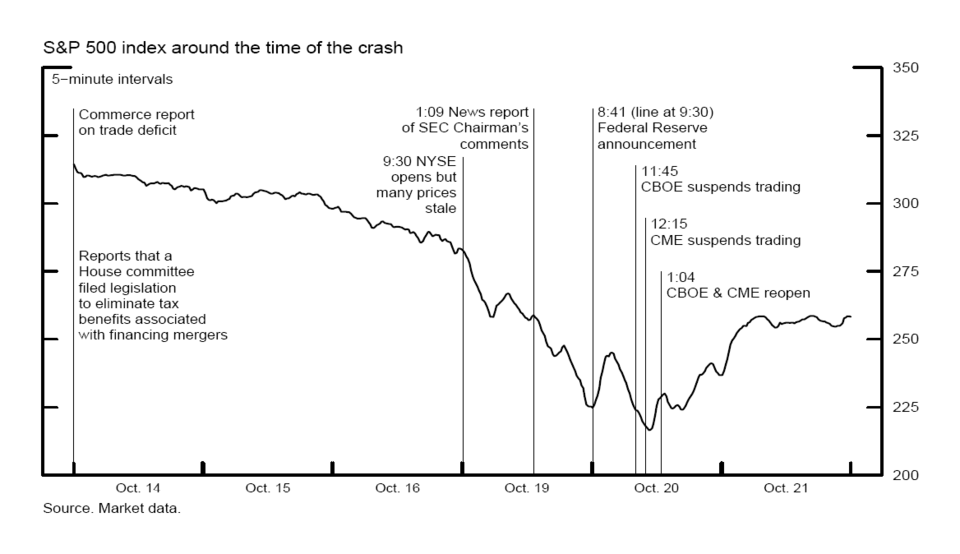
\includegraphics[height=0.36\textheight]{ch11_sp500_1987_fed.png}\\[1mm]
\imgcap{S\&P 500 în jurul crahului din octombrie 1987}
\imgcredit{https://commons.wikimedia.org/wiki/File:S\%26P_500_index_around_the_time_of_the_crash.png}{Grafic: Mark Carlson, Federal Reserve Board (2006); domeniu public; Wikimedia Commons}
\end{column}
\end{columns}
\end{frame}

\begin{frame}{Testarea FMH: scalare, orizonturi și lichiditate}
\itemsize{\small}
\begin{itemize}
    \item FMH este o teorie formulată verbal; consecințele ei statistice pot fi testate
    \begin{itemize}
        \item \textbf{autosimilaritate}: distribuția randamentelor pe $h$ zile arată la fel după rescalarea cu $h^H$ (secțiunea 2)
        \item \textbf{memorie}: exponentul Hurst $H$ măsoară dependența pe orizonturi lungi (secțiunile 3--5)
        \item \textbf{schimbare}: în crize, $H$ și ponderea orizonturilor scurte ar trebui să se schimbe (secțiunea 8)
    \end{itemize}
    \item Studii de referință: \refKrisA\ și \refKrisB\ despre criza din 2008
    \begin{itemize}
        \item exponenți Hurst locali și puterea wavelet a indicilor din SUA și Europa
        \item perioadele cele mai turbulente coincid cu dominația orizonturilor investiționale scurte, așa cum prezice FMH
    \end{itemize}
\end{itemize}
\end{frame}

\begin{frame}{EMH, FMH și AMH}
\itemsize{\small}
\begin{center}
\footnotesize
\begin{tabular}{>{\raggedright\arraybackslash}p{2.2cm}>{\raggedright\arraybackslash}p{2.9cm}>{\raggedright\arraybackslash}p{2.9cm}>{\raggedright\arraybackslash}p{2.9cm}}
\toprule
 & \textbf{EMH} & \textbf{FMH} & \textbf{AMH} \\
\midrule
Sursa & \refFama{} & \refPeters{} & \refLoAMH{} \\
Investitorii & un investitor reprezentativ & multe orizonturi & specii care concurează și se adaptează \\
Stabilitatea & prețuri mereu corecte & diversitatea orizonturilor aduce lichiditate & se schimbă odată cu mediul \\
Memoria & $H = 0{,}5$ & $H$ poate fi diferit de 0,5 & $H$ variază în timp \\
Crizele & în afara teoriei & prăbușirea orizonturilor & dispariția în masă a strategiilor \\
\bottomrule
\end{tabular}
\end{center}
\begin{itemize}
    \item Cele trei nu sînt teste rivale: FMH și AMH explică unde și de ce aproximarea EMH nu mai funcționează
\end{itemize}
\end{frame}

\begin{frame}{Recapitulare: de la piețe eficiente la piețe fractale}
\itemsize{\small}
\begin{itemize}
    \item FMH: stabilitatea vine de la investitori cu orizonturi diferite, care își oferă lichiditate unii altora
    \item Crahurile: orizonturile se reduc la un singur orizont scurt
    \item Testabilă prin scalare și memorie, măsurate de exponentul Hurst $H$
\end{itemize}
\end{frame}


%=============================================================================
\section{Autosimilaritate și fractali}
%=============================================================================

\begin{frame}{Benoît Mandelbrot: rugozitatea ca măsură}
\itemsize{\footnotesize}
\begin{columns}[T]
\begin{column}{0.58\textwidth}
\begin{itemize}
    \item \refMan: prețurile bumbacului au cozi groase și arată asemănător la scară zilnică, lunară și anuală
    \begin{itemize}
        \item distribuțiile $\alpha$-stabile din \sfmchlink{https://danpele.github.io/SFM/RO/Cursuri/capitol3_distributii_alfa_stabile.pdf}{Capitolul 3}
    \end{itemize}
    \item \refCoast: lungimea măsurată a unei coaste crește cînd rigla devine mai mică; rata de creștere definește o \textbf{dimensiune fractală}
    \item \refMVN: mișcarea browniană fracționară, modelul acestui capitol
    \item \textbf{Fractal}: un obiect ale cărui părți seamănă cu întregul, exact sau în distribuție
\end{itemize}
\end{column}
\begin{column}{0.38\textwidth}
\centering
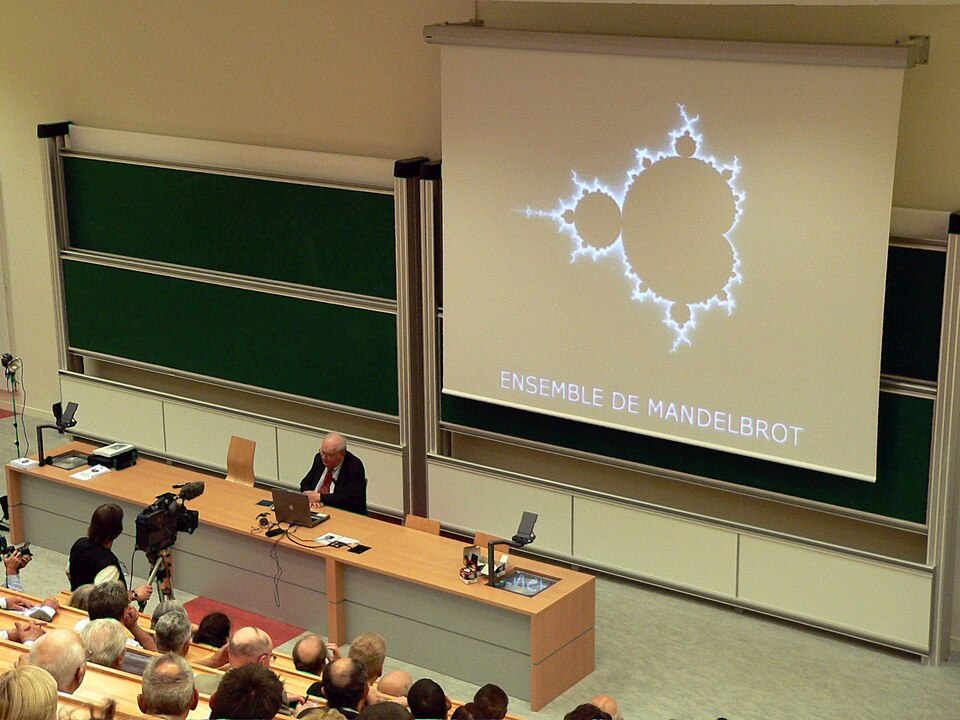
\includegraphics[height=0.25\textheight]{ch11_mandelbrot_2006.jpg}\\[1mm]
\imgcap{Benoît Mandelbrot (1924--2010), Paris, 2006}
\imgcredit{https://commons.wikimedia.org/wiki/File:Mandelbrot_p1130876.jpg}{Foto: David Monniaux (2006); CC BY-SA 3.0; Wikimedia Commons}\\[1mm]
\centering

\includegraphics[height=0.15\textheight]{ch11_mandelbrot_set.jpg}\\[1mm]
\imgcap{Mulțimea Mandelbrot}
\imgcredit{https://commons.wikimedia.org/wiki/File:Mandel_zoom_00_mandelbrot_set.jpg}{Imagine: Wolfgang Beyer; CC BY-SA 3.0; Wikimedia Commons}
\end{column}
\end{columns}
\end{frame}

\begin{frame}{Dimensiunea fractală}
\itemsize{\small}
\begin{itemize}
    \item \textbf{Dimensiunea de similaritate}: un obiect format din $N$ copii ale lui însuși, fiecare scalată cu $1/s$, are $D = \ln N/\ln s$
    \begin{itemize}
        \item un segment: 2 jumătăți, $D = \ln 2/\ln 2 = 1$; un pătrat: 4 sferturi cu latura $1/2$, $D = \ln 4/\ln 2 = 2$
        \item curba Koch: 4 copii scalate cu $1/3$, $D = \ln 4/\ln 3 = 1{,}262$
        \item triunghiul Sierpinski: 3 copii scalate cu $1/2$, $D = \ln 3/\ln 2 = 1{,}585$
    \end{itemize}
    \item Coasta de vest a Marii Britanii: $D \approx 1{,}25$ \refCoast
    \item Graficul unei traiectorii de preț: $D = 2 - H$
    \begin{itemize}
        \item mișcarea browniană: $D = 1{,}5$; o traiectorie mai netedă, cu tendințe ($H > 0{,}5$), are $D < 1{,}5$
    \end{itemize}
\end{itemize}
\end{frame}

\begin{frame}{Procese autosimilare}
\itemsize{\small}
\begin{itemize}
    \item \textbf{Proces autosimilar} \refFHH, Def.~14.1: $X_{ct} \overset{d}{=} c^H X_t$ pentru orice $c > 0$; $H$ este \textbf{exponentul Hurst}
    \begin{itemize}
        \item $\overset{d}{=}$: egalitate în distribuție; dilatarea timpului cu $c$ echivalează cu dilatarea valorilor cu $c^H$
    \end{itemize}
    \item Mișcarea browniană (\sfmchlink{https://danpele.github.io/SFM/RO/Cursuri/capitol4_probabilitate.pdf}{Capitolul 4}) este autosimilară cu $H = 1/2$: $W_{ct} \overset{d}{=} \sqrt{c}\,W_t$
    \item Consecință pentru prețurile logaritmice cu creșteri autosimilare
    \begin{itemize}
        \item $\mathrm{sd}(r_t^{(h)}) = h^H\,\mathrm{sd}(r_t)$, unde $r_t^{(h)}$ este randamentul pe $h$ zile
        \item regula rădăcinii pătrate a timpului, $\sqrt{h}$, este cazul particular $H = 1/2$
    \end{itemize}
    \item Un prim estimator al lui $H$: panta dreptei lui $\ln \mathrm{sd}(r^{(h)})$ în funcție de $\ln h$
\end{itemize}
\end{frame}

\begin{frame}{Scalarea randamentelor pe $h$ zile}
\itemsize{\footnotesize}
\begin{center}
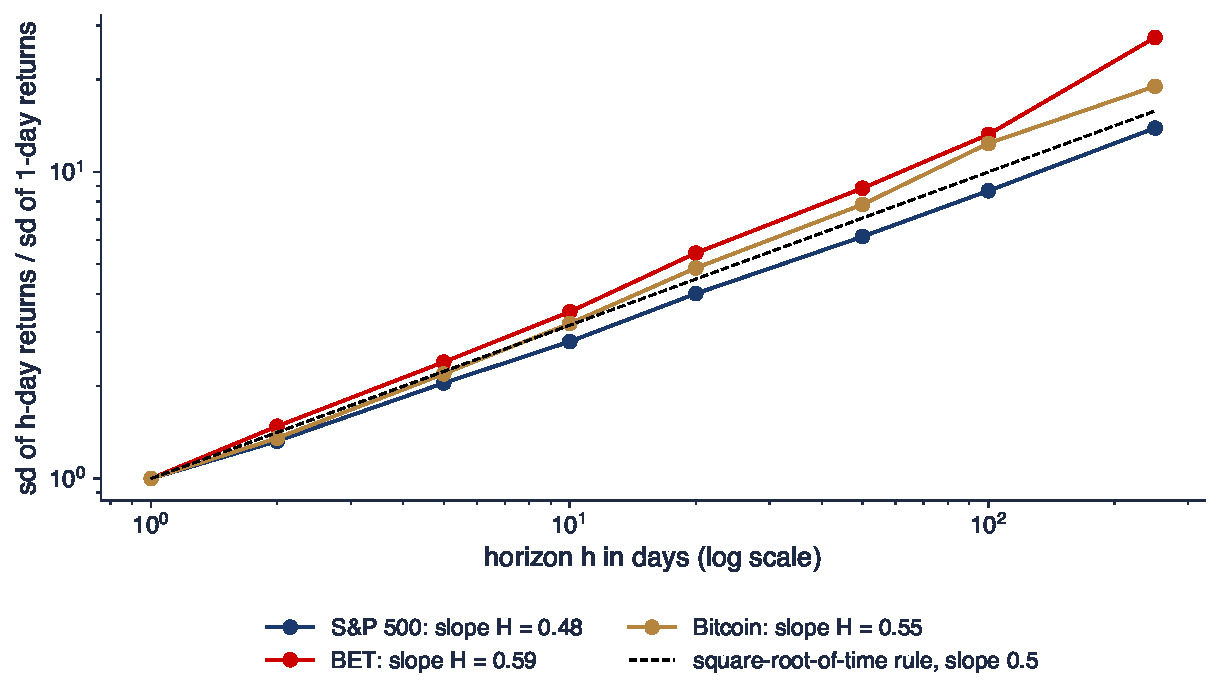
\includegraphics[width=0.97\textwidth,height=0.50\textheight,keepaspectratio]{sfm_ch11_scaling.pdf}
\end{center}
\vspace{-0.25cm}
\begin{itemize}
    \item Abaterea standard a randamentelor pe $h$ zile, fără suprapunere, împărțită la cea zilnică, $h = 1, \dots, 250$, scale logaritmice; date pînă la 18 septembrie 2026
    \item Pante: S\&P 500 $0{,}48$, BET $0{,}59$, Bitcoin $0{,}55$; regula rădăcinii pătrate are panta 0,5
\end{itemize}
\sfmquantlet{Ch_11}{SFM_ch11_self_similarity}
\end{frame}

\begin{frame}{Interpretarea exponenților de scalare}
\itemsize{\small}
\begin{itemize}
    \item S\&P 500: riscul pe 10 zile este de $2{,}80$ ori riscul zilnic, sub $\sqrt{10} = 3{,}16$
    \begin{itemize}
        \item ușoară revenire la medie: randamentele zilnice au autocorelația de ordinul întîi negativă, $-0{,}099$
    \end{itemize}
    \item BET: de $3{,}50$ ori, peste $\sqrt{10}$: autocorelație pozitivă
    \begin{itemize}
        \item tranzacționarea redusă din primii ani face ca indicele să se ajusteze lent (\sfmchlink{https://danpele.github.io/SFM/RO/Cursuri/capitol7_piete_eficiente_mers_aleator_vr.pdf}{Capitolul 7})
    \end{itemize}
    \item Bitcoin: de $3{,}20$ ori, aproape de $\sqrt{10}$
    \item Atenție: există doar cîteva zeci de blocuri de 250 de zile fără suprapunere; panta este imprecisă, deci avem nevoie de un estimator adecvat și de o bandă de încredere
\end{itemize}
\end{frame}

\begin{frame}{Recapitulare: autosimilaritate și fractali}
\itemsize{\small}
\begin{itemize}
    \item Fractal: părțile seamănă cu întregul; dimensiunea fractală $D = \ln N/\ln s$
    \item Proces autosimilar: $X_{ct} \overset{d}{=} c^H X_t$; mișcarea browniană are $H = 1/2$
    \item Riscul se scalează ca $h^H$; regula $\sqrt{h}$ presupune $H = 1/2$
\end{itemize}
\end{frame}


%=============================================================================
\section{Hurst, Nilul și statistica R/S}
%=============================================================================

\begin{frame}{Harold Edwin Hurst și Nilul}
\itemsize{\footnotesize}
\begin{columns}[T]
\begin{column}{0.60\textwidth}
\begin{itemize}
    \item Hurst (1880--1978), hidrolog britanic care a lucrat în Egipt din 1906, a proiectat rezervoare pe Nil
    \begin{itemize}
        \item capacitatea necesară pentru a livra în fiecare an debitul mediu este egală cu amplitudinea abaterilor cumulate ale debitelor de la medie
    \end{itemize}
    \item \refHurst: pentru debite independente, această amplitudine crește ca $n^{0{,}5}$; în seriile de debite ale rîurilor, de precipitații și de inele ale copacilor crește ca $n^{K}$, cu $K$ în medie de circa $0{,}73$
    \begin{itemize}
        \item anii cu debit mare urmează după ani cu debit mare: \textbf{memorie lungă}
    \end{itemize}
\end{itemize}
\end{column}
\begin{column}{0.36\textwidth}
\centering
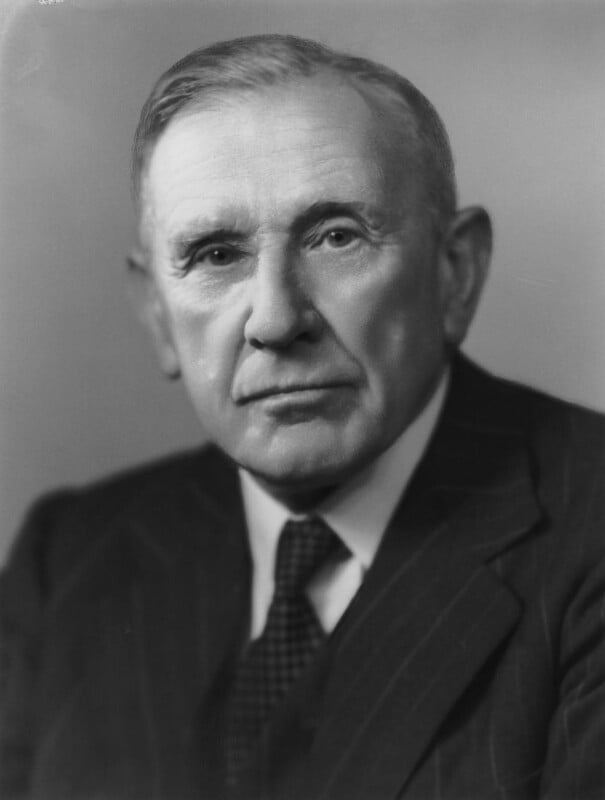
\includegraphics[height=0.24\textheight]{ch11_hurst_1953.jpg}\\[1mm]
\imgcap{H.E. Hurst (1953)}
\imgcredit{https://commons.wikimedia.org/wiki/File:Harold_Edwin_Hurst_in_1953.jpg}{Foto: Elliott \& Fry (1953); domeniu public; Wikimedia Commons}\\[1mm]
\centering
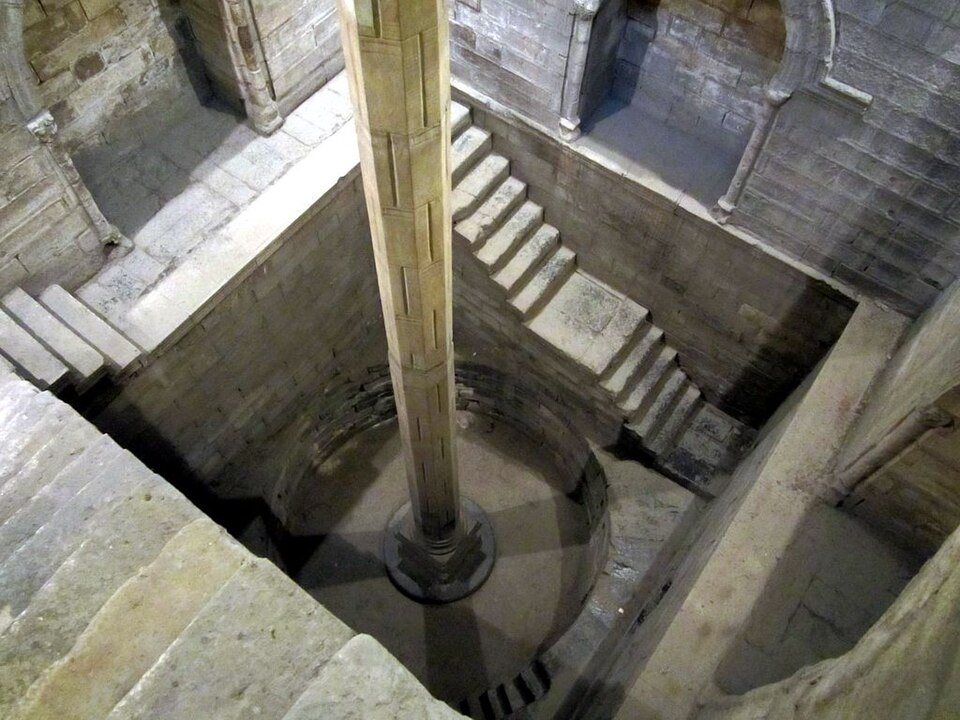
\includegraphics[height=0.17\textheight]{ch11_nilometer_roda.jpg}\\[1mm]
\imgcap{Nilometrul de pe insula Roda, Cairo, construit în 861}
\imgcredit{https://commons.wikimedia.org/wiki/File:Nilometer_(8590204613).jpg}{Foto: David Stanley (2013); CC BY 2.0; Wikimedia Commons}
\end{column}
\end{columns}
\end{frame}

\begin{frame}{Statistica R/S}
\itemsize{\small}
\begin{itemize}
    \item Blocul $x_1, \dots, x_n$, cu media $\bar x$; \textbf{abaterile cumulate} $Y_k = \sum_{j=1}^{k}(x_j - \bar x)$, $k = 1, \dots, n$
    \begin{itemize}
        \item $Y_n = 0$ prin construcție
    \end{itemize}
    \item \textbf{Amplitudinea}: $R_n = \max_k Y_k - \min_k Y_k$; \textbf{abaterea standard}: $S_n = \sqrt{\tfrac1n\sum_j (x_j - \bar x)^2}$
    \item \textbf{Statistica R/S} (rescaled range, amplitudinea rescalată) \refFHH, 14.4.1: $(R/S)_n = R_n/S_n$
    \begin{itemize}
        \item împărțirea la $S_n$ elimină unitatea de măsură: $(R/S)_n$ este comparabilă între active
        \item pentru date i.i.d.\ cu varianță finită, $(R/S)_n$ crește ca $n^{1/2}$; sub memorie lungă crește ca $n^H$, $H > 1/2$
    \end{itemize}
    \item Robustă la cozi groase: $R$ și $S$ sînt mărite de aceleași valori extreme \refMW
\end{itemize}
\end{frame}

\begin{frame}{Exemplu lucrat: R/S pentru opt randamente}
\itemsize{\scriptsize}
\begin{columns}[T]
\begin{column}{0.52\textwidth}
\begin{itemize}
    \item Randamente (\%): $0{,}5;\ -0{,}3;\ 0{,}8;\ -0{,}2;\ 0{,}6;\ -0{,}1;\ 0{,}4;\ -0{,}7$
    \item Media $\bar x = 1{,}0/8 = 0{,}125$
    \item Abateri: $+0{,}375$; $-0{,}425$; $+0{,}675$; $-0{,}325$; $+0{,}475$; $-0{,}225$; $+0{,}275$; $-0{,}825$
    \item $Y_k$: $0{,}375$; $-0{,}050$; $0{,}625$; $0{,}300$; $0{,}775$; $0{,}550$; $0{,}825$; $0{,}000$
    \item $R = 0{,}825 - (-0{,}050) = 0{,}875$; $S = \sqrt{1{,}915/8} = 0{,}489$
    \item $(R/S)_8 = 0{,}875/0{,}489 = 1{,}788$; un bloc dă un singur punct, iar $H$ are nevoie de multe mărimi de bloc
\end{itemize}
\end{column}
\begin{column}{0.46\textwidth}
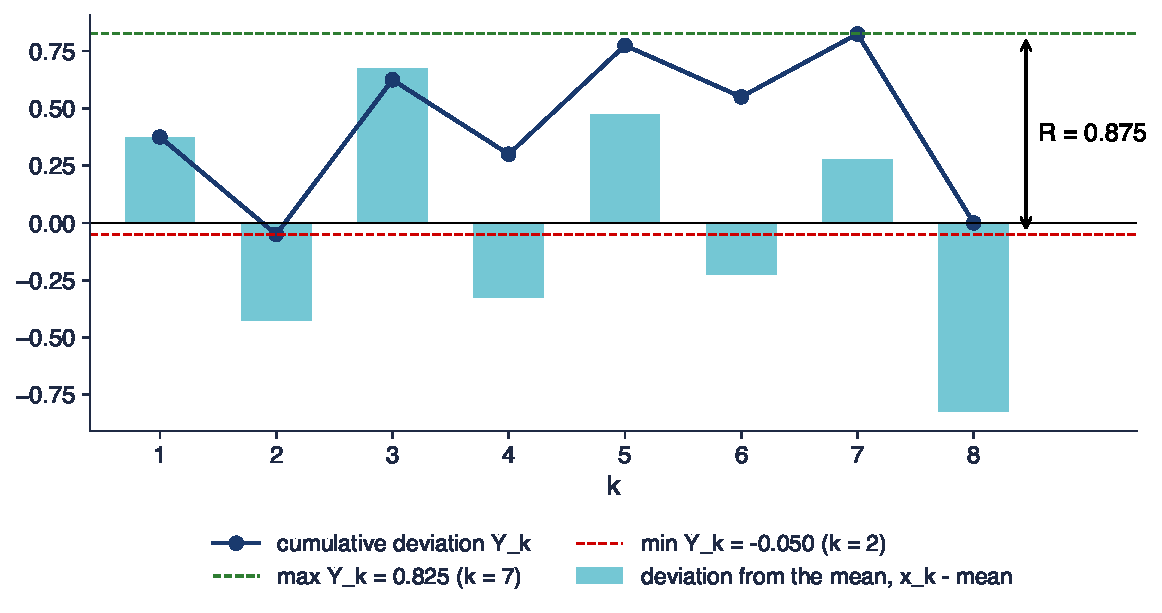
\includegraphics[width=\textwidth]{sfm_ch11_rs_example.pdf}
\sfmquantlet{Ch_11}{SFM_ch11_rs_estimators}
\end{column}
\end{columns}
\end{frame}

\begin{frame}{De la R/S la exponentul Hurst}
\itemsize{\small}
\begin{itemize}
    \item Pașii \refMW
    \begin{itemize}
        \item alegem mărimi de bloc $n$ între 10 și $N/4$, la distanțe egale pe scară logaritmică
        \item împărțim cele $N$ randamente în $\lfloor N/n\rfloor$ blocuri fără suprapunere; calculăm $R/S$ în fiecare bloc și facem media: $(R/S)_n$
        \item estimăm prin OLS (ordinary least squares, metoda celor mai mici pătrate) $\ln (R/S)_n = \ln c + H \ln n + e_n$: panta $\hat H$ estimează $H$
    \end{itemize}
    \item Graficul log-log este principalul instrument de diagnostic: o dreaptă susține existența unui singur exponent de scalare
    \item Se aplică randamentelor (staționare), nu prețurilor: pentru prețuri, $(R/S)_n$ crește ca $n$
\end{itemize}
\end{frame}

\begin{frame}{Interpretarea exponentului $H$}
\itemsize{\small}
\begin{center}
\footnotesize
\begin{tabular}{llll}
\toprule
$H$ & creșteri & memorie & traiectorie ($D = 2 - H$) \\
\midrule
$0 < H < 0{,}5$ & corelate negativ & antipersistentă: inversări & rugoasă, $D > 1{,}5$ \\
$H = 0{,}5$ & necorelate & fără memorie (mers aleator) & $D = 1{,}5$ \\
$0{,}5 < H < 1$ & corelate pozitiv & persistentă: tendințe & mai netedă, $D < 1{,}5$ \\
\bottomrule
\end{tabular}
\end{center}
\begin{itemize}
    \item $H$ nu este o probabilitate: $H = 0{,}7$ nu înseamnă „70\% șanse ca semnul să se repete”
    \item Două efecte numite de \refNoah
    \begin{itemize}
        \item \textbf{efectul Noe}: valori extreme (cozi groase, potopul); \textbf{efectul Iosif}: serii lungi de valori mari sau mici („șapte ani de belșug, șapte ani de foamete”)
        \item $H$ măsoară efectul Iosif; indicele de coadă din \sfmchlink{https://danpele.github.io/SFM/RO/Cursuri/capitol5_cozi_groase_evt.pdf}{Capitolul 5} măsoară efectul Noe
    \end{itemize}
\end{itemize}
\end{frame}

\begin{frame}{Eșantioane mici: deplasarea estimatorului R/S}
\itemsize{\small}
\begin{itemize}
    \item Pentru date i.i.d., $(R/S)_n$ se apropie de $c\,n^{1/2}$ doar pentru $n$ mare; pentru $n$ mic crește mai repede \refAL
    \begin{itemize}
        \item panta estimată pe $n = 10, \dots, N/4$ este peste 0,5 chiar fără nicio memorie
    \end{itemize}
    \item Monte Carlo, 500 de serii i.i.d.\ Normale
    \begin{itemize}
        \item $\hat H_{R/S}$ mediu: $0{,}588$ pentru $N = 250$, $0{,}562$ pentru $N = 1000$, $0{,}547$ pentru $N = 5000$
        \item banda de 95\% pentru $N = 1000$: $[0{,}50; 0{,}63]$
    \end{itemize}
    \item Regulă: comparăm $\hat H$ cu distribuția lui $\hat H$ sub ipoteza nulă, pentru același $N$, nu cu 0,5 (secțiunea 5)
\end{itemize}
\end{frame}

\begin{frame}{Recapitulare: Hurst, Nilul și statistica R/S}
\itemsize{\small}
\begin{itemize}
    \item $(R/S)_n$: amplitudinea abaterilor cumulate împărțită la abaterea standard
    \item $\hat H$ = panta lui $\ln(R/S)_n$ în funcție de $\ln n$; 0,5: fără memorie, peste: persistență, sub: antipersistență
    \item R/S este deplasat în sus în eșantioane mici: comparăm cu o bandă Monte Carlo
\end{itemize}
\end{frame}


%=============================================================================
\section{Memoria lungă: definiții și modele}
%=============================================================================

\begin{frame}{Memorie scurtă și memorie lungă}
\itemsize{\small}
\begin{itemize}
    \item $X_t$ staționar, cu autocorelațiile $\rho(k)$ (ACF, autocorrelation function, funcția de autocorelație); \textbf{memorie lungă} \refFHH, 14.1:
    \begin{itemize}
        \item $\sum_{k} |\rho(k)| = \infty$: autocorelațiile nu sînt sumabile
        \item echivalent, scădere hiperbolică $\rho(k) \sim C\,k^{2d - 1}$ cînd $k \to \infty$, cu \textbf{parametrul de memorie} $0 < d < 0{,}5$
        \item în frecvență: densitatea spectrală are un pol în zero, $f(\lambda) \sim C\,\lambda^{-2d}$ cînd $\lambda \to 0$
    \end{itemize}
    \item \textbf{Memorie scurtă}: modelele ARMA (autoregressive moving average, autoregresive cu medie mobilă), de exemplu AR(1) cu $\rho(k) = \phi^k$
    \begin{itemize}
        \item scădere exponențială: $\sum_k |\phi|^k = 1/(1 - |\phi|) < \infty$
    \end{itemize}
    \item Legătura cu exponentul Hurst: $d = H - 1/2$
\end{itemize}
\end{frame}

\begin{frame}{Exemplu lucrat: cît de repede se stinge memoria?}
\itemsize{\small}
\begin{itemize}
    \item Memorie lungă: zgomot gaussian fracționar (slide-urile următoare) cu $H = 0{,}8$
    \begin{itemize}
        \item $\rho(1) = 2^{2H - 1} - 1 = 2^{0{,}6} - 1 = 0{,}516$
        \item $\rho(10) = 0{,}191$, $\rho(50) = 0{,}100$, $\rho(100) = 0{,}076$
    \end{itemize}
    \item Memorie scurtă: AR(1) cu aceeași autocorelație de ordinul întîi, $\phi = 0{,}516$
    \begin{itemize}
        \item $\rho(10) = \phi^{10} = 0{,}0013$; $\rho(100) = \phi^{100}$, practic zero
    \end{itemize}
    \item Același comportament pe termen scurt, dar un termen lung foarte diferit: după 100 de zile, un șoc mai contează doar sub memorie lungă
\end{itemize}
\end{frame}

\begin{frame}{Mișcarea browniană fracționară}
\itemsize{\small}
\begin{itemize}
    \item \textbf{Mișcarea browniană fracționară} (fBm, fractional Brownian motion) $B_H(t)$, $0 < H < 1$ \refMVN; \refFHH, Def.~14.2: proces gaussian cu traiectorii continue, autosimilar cu exponentul $H$ și cu creșteri staționare
    \item Proprietăți (\refFHH, Teorema 14.1)
    \begin{itemize}
        \item $B_H(0) = 0$, $E[B_H(t)] = 0$, $E[B_H(t)^2] = \sigma^2 |t|^{2H}$
        \item $\mathrm{Cov}(B_H(t), B_H(s)) = \tfrac{\sigma^2}{2}\left(|t|^{2H} + |s|^{2H} - |t - s|^{2H}\right)$
    \end{itemize}
    \item $H = 1/2$: mișcarea browniană, creșteri independente; $H \neq 1/2$: creșterile sînt corelate la toate decalajele
    \item Simulare: exactă, din matricea de covarianță a creșterilor (scufundare circulantă, ca în notebook)
\end{itemize}
\end{frame}

\begin{frame}{Traiectorii fBm pentru trei exponenți Hurst}
\itemsize{\footnotesize}
\begin{center}
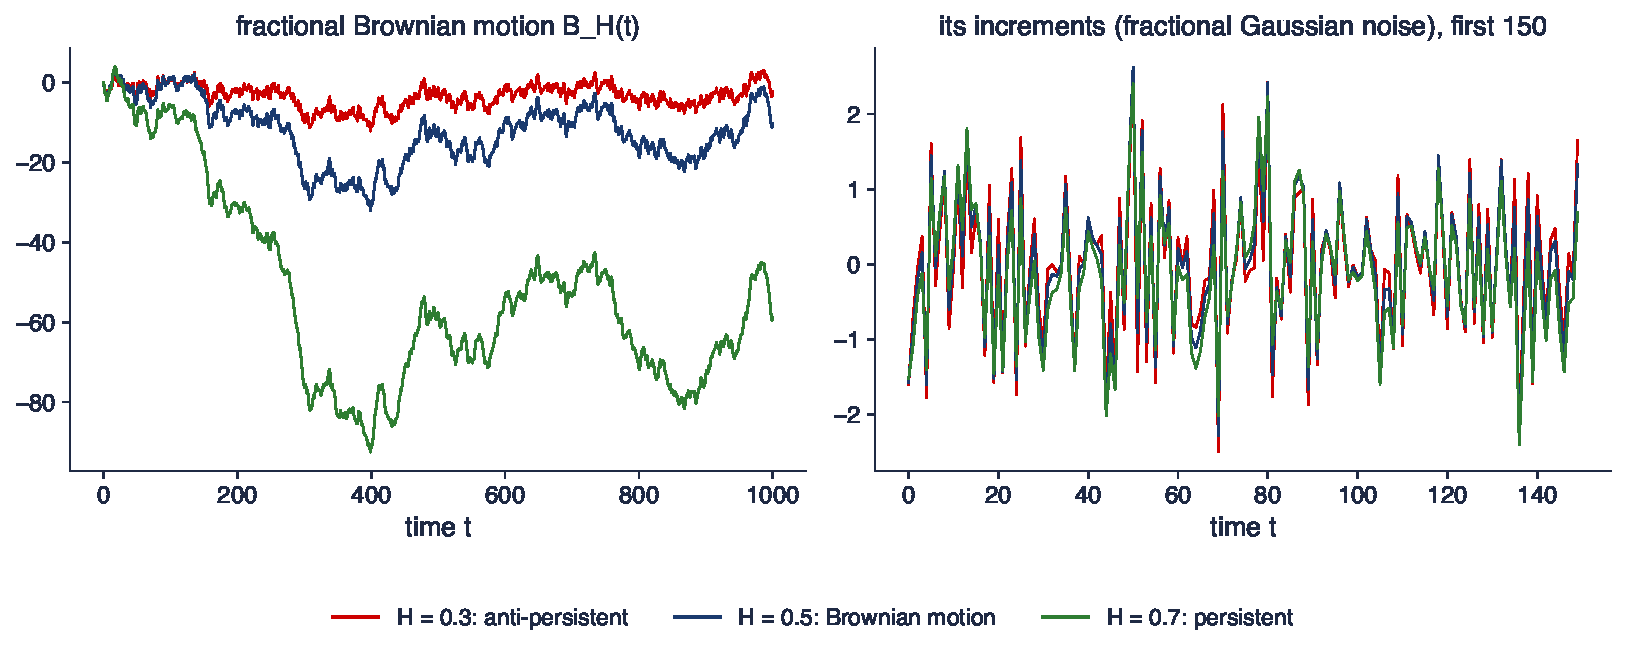
\includegraphics[width=0.97\textwidth,height=0.52\textheight,keepaspectratio]{sfm_ch11_fbm_paths.pdf}
\end{center}
\vspace{-0.25cm}
\begin{itemize}
    \item Aceleași numere aleatoare, $H = 0{,}3$, $0{,}5$, $0{,}7$ (ca în SFEfbmplot); dreapta: primele 150 de creșteri
    \item $H = 0{,}7$: excursii lungi și amplitudine mare; $H = 0{,}3$: inversări frecvente, amplitudine mică; autocorelația de ordinul 1 a creșterilor $0{,}32$ și $-0{,}23$ (teoretic $0{,}32$ și $-0{,}24$)
\end{itemize}
\sfmquantlet{Ch_11}{SFM_ch11_fbm_fgn}
\end{frame}

\begin{frame}{Zgomotul gaussian fracționar}
\itemsize{\small}
\begin{itemize}
    \item \textbf{Zgomotul gaussian fracționar} (fGn, fractional Gaussian noise): creșterile $Y_k = B_H(k + 1) - B_H(k)$, o serie staționară \refFHH, 14.3
    \begin{itemize}
        \item $\rho(k) = \tfrac12\left(|k + 1|^{2H} - 2|k|^{2H} + |k - 1|^{2H}\right)$
        \item pentru $k$ mare: $\rho(k) \approx H(2H - 1)\,k^{2H - 2}$
    \end{itemize}
    \item Trei regimuri
    \begin{itemize}
        \item $1/2 < H < 1$: $\rho(k) > 0$ și nesumabile: memorie lungă cu $d = H - 1/2 \in (0, 1/2)$
        \item $H = 1/2$: zgomot alb
        \item $0 < H < 1/2$: $\rho(k) < 0$, sumabile: antipersistență
    \end{itemize}
    \item fGn este modelul din spatele R/S și DFA: pentru date fGn, ambele estimează $H$
\end{itemize}
\end{frame}

\begin{frame}{ACF a zgomotului gaussian fracționar}
\itemsize{\footnotesize}
\begin{center}
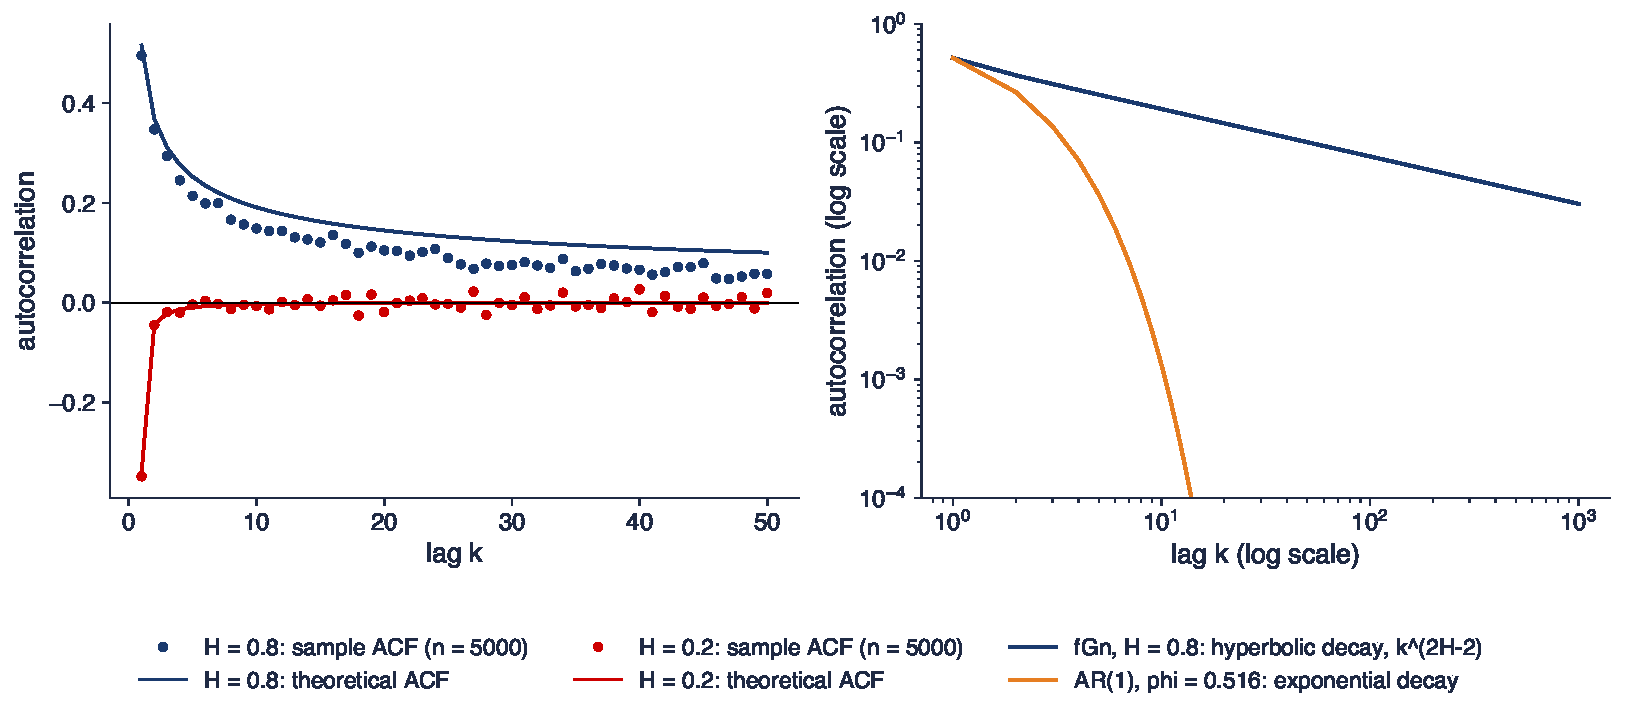
\includegraphics[width=0.97\textwidth,height=0.48\textheight,keepaspectratio]{sfm_ch11_fgn_acf.pdf}
\end{center}
\vspace{-0.25cm}
\begin{itemize}
    \item Stînga: ACF de selecție și teoretică pentru $H = 0{,}8$ și $H = 0{,}2$ (ca în SFEfgnacf); $\rho(1) = 0{,}516$ și $-0{,}340$
    \item Dreapta, scale logaritmice: scădere hiperbolică (o dreaptă) față de scăderea exponențială a unui AR(1) cu același $\rho(1)$
    \item ACF de selecție a unei serii cu memorie lungă este sub cea teoretică: estimarea mediei elimină o parte din componenta lentă
\end{itemize}
\sfmquantlet{Ch_11}{SFM_ch11_fbm_fgn}
\end{frame}

\begin{frame}{ARFIMA(0,$d$,0): diferențierea fracționară}
\itemsize{\footnotesize}
\begin{itemize}
    \item \textbf{ARFIMA}(0,$d$,0) \refGJ; \refHosking: $(1 - L)^d X_t = \varepsilon_t$, $\varepsilon_t$ i.i.d.\ $(0, \sigma^2)$, $L$ operatorul de decalaj ($L X_t = X_{t-1}$)
    \begin{itemize}
        \item ARFIMA: autoregressive fractionally integrated moving average, model autoregresiv fracționar integrat cu medie mobilă; $d = 0$: zgomot alb, $d = 1$: mers aleator (\sfmchlink{https://danpele.github.io/SFM/RO/Cursuri/capitol7_piete_eficiente_mers_aleator_vr.pdf}{Capitolul 7})
    \end{itemize}
    \item Dezvoltarea binomială \refFHH, 14.2: $(1 - L)^d = \sum_{j \ge 0} \pi_j L^j$, $\pi_0 = 1$, $\pi_j = \pi_{j-1}\,(j - 1 - d)/j$
    \begin{itemize}
        \item $X_t = \varepsilon_t - \sum_{j \ge 1}\pi_j X_{t-j}$: contează tot trecutul, cu ponderi care scad lent
        \item forma MA($\infty$): $X_t = \sum_{j \ge 0}\psi_j\varepsilon_{t-j}$, $\psi_0 = 1$, $\psi_j = \psi_{j-1}\,(j - 1 + d)/j$
    \end{itemize}
    \item Autocorelațiile: $\rho(k) = \dfrac{\Gamma(1 - d)\,\Gamma(k + d)}{\Gamma(d)\,\Gamma(k + 1 - d)}$, adică $\rho(k) = \rho(k - 1)\,\dfrac{k - 1 + d}{k - d}$
    \begin{itemize}
        \item $\rho(1) = d/(1 - d)$; pentru $k$ mare, $\rho(k) \sim C k^{2d - 1}$: memorie lungă pentru $0 < d < 1/2$
    \end{itemize}
\end{itemize}
\end{frame}

\begin{frame}{Parametrul de memorie $d$}
\itemsize{\small}
\begin{center}
\footnotesize
\begin{tabular}{lllll}
\toprule
$d$ & memorie & revenire la medie & varianță & ACF \\
\midrule
$(-0{,}5; 0)$ & antipersistentă & da & finită & hiperbolică, negativă \\
$0$ & scurtă & da & finită & exponențială (ARMA) \\
$(0; 0{,}5)$ & lungă, staționară & da & finită & hiperbolică \\
$[0{,}5; 1)$ & lungă, nestaționară & da & infinită & hiperbolică \\
$1$ & rădăcină unitară & nu & infinită & nu scade \\
\bottomrule
\end{tabular}
\end{center}
\begin{itemize}
    \item Sursa: \refFHH, tabelul 14.1; $H = d + 1/2$ pe domeniul staționar
    \item ARFIMA($p$,$d$,$q$): dinamica ARMA($p$,$q$) pentru termen scurt, $d$ pentru termen lung \refFHH, 14.6.1
    \item Integrarea fracționară acoperă spațiul dintre cazul staționar $d = 0$ și rădăcina unitară $d = 1$ din \sfmchlink{https://danpele.github.io/SFM/RO/Cursuri/capitol7_piete_eficiente_mers_aleator_vr.pdf}{Capitolul 7}
\end{itemize}
\end{frame}

\begin{frame}{ARFIMA(0,$d$,0) cu $d = 0{,}4$ și $d = -0{,}4$}
\itemsize{\footnotesize}
\begin{center}
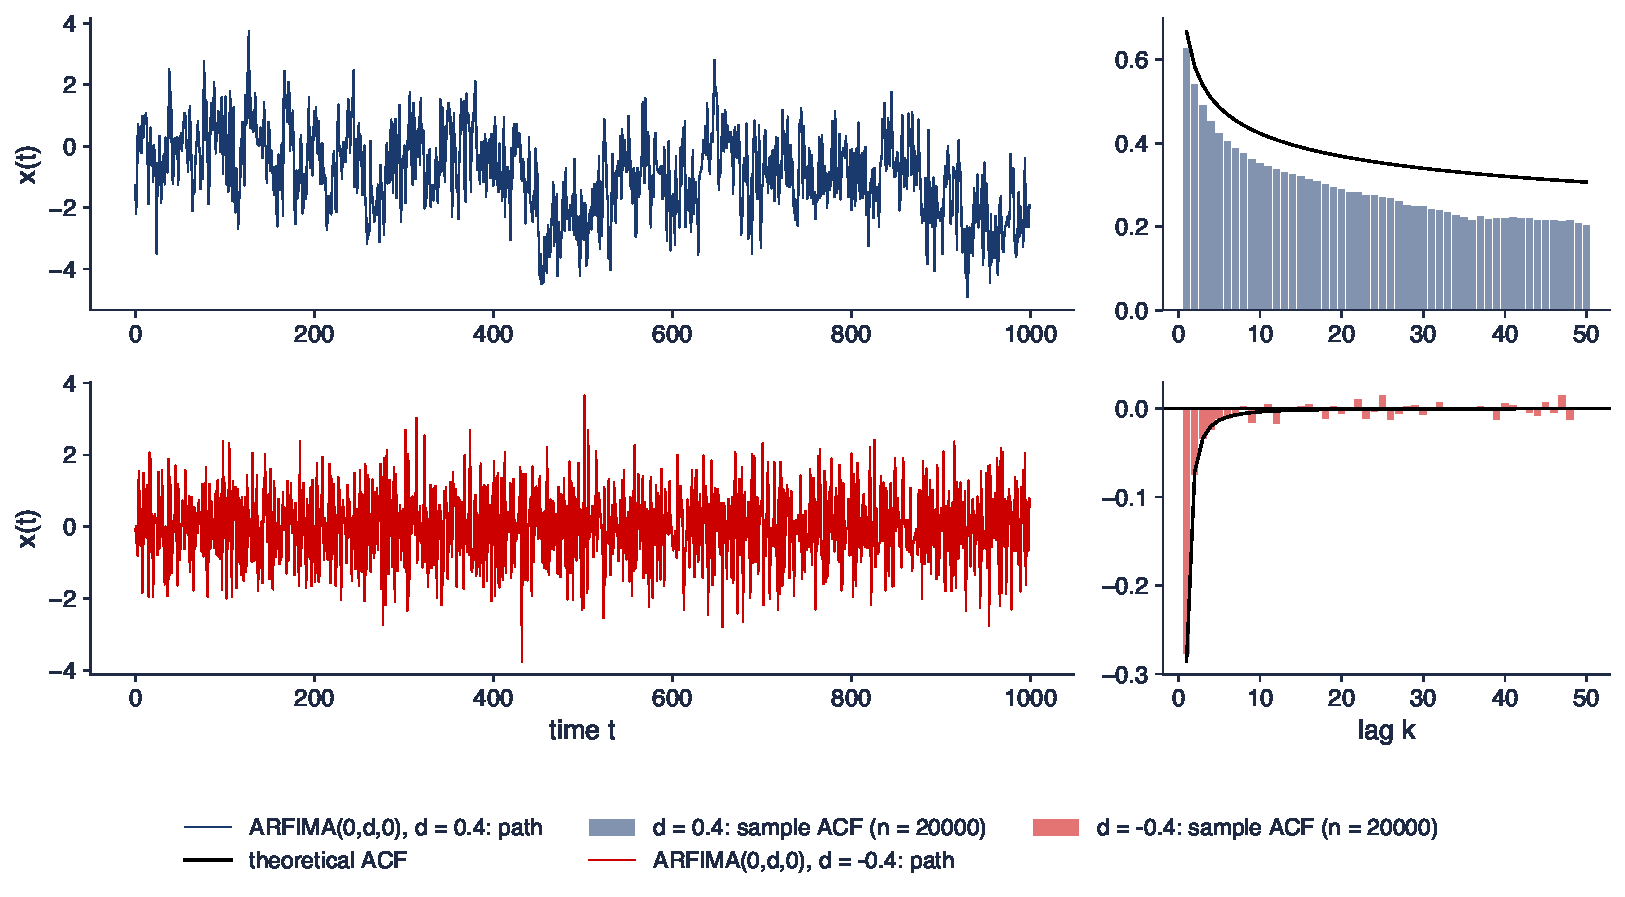
\includegraphics[width=0.97\textwidth,height=0.52\textheight,keepaspectratio]{sfm_ch11_arfima.pdf}
\end{center}
\vspace{-0.25cm}
\begin{itemize}
    \item Stînga: 1000 de valori simulate (ca în SFEarfima); dreapta: ACF de selecție (20000 de valori) și ACF teoretică
    \item $d = 0{,}4$: $\rho(1) = 0{,}667$, $\rho(10) = 0{,}424$, $\rho(50) = 0{,}307$: valuri lente în jurul mediei; $d = -0{,}4$: $\rho(1) = -0{,}286$, apoi aproape zero
\end{itemize}
\sfmquantlet{Ch_11}{SFM_ch11_arfima}
\end{frame}

\begin{frame}{Exemplu lucrat: ARFIMA(0; 0,3; 0)}
\itemsize{\small}
\begin{itemize}
    \item Ponderile lui $(1 - L)^{0{,}3}$: $\pi_1 = -d = -0{,}300$, $\pi_2 = \pi_1(1 - d)/2 = -0{,}105$
    \begin{itemize}
        \item ponderile MA: $\psi_1 = d = 0{,}300$, $\psi_2 = \psi_1(1 + d)/2 = 0{,}195$
    \end{itemize}
    \item Autocorelațiile
    \begin{itemize}
        \item $\rho(1) = 0{,}3/0{,}7 = 0{,}429$; $\rho(2) = \rho(1) \times 1{,}3/1{,}7 = 0{,}328$
        \item $\rho(10) = 0{,}173$, $\rho(100) = 0{,}069$
    \end{itemize}
    \item AR(1) cu $\phi = 0{,}429$: $\rho(10) = 0{,}0002$
    \item Autocorelația scade sub 0,05 după 4 decalaje pentru AR(1) și după 222 de decalaje pentru ARFIMA; $H = d + 0{,}5 = 0{,}8$
\end{itemize}
\end{frame}

\begin{frame}{Recapitulare: memoria lungă}
\itemsize{\small}
\begin{itemize}
    \item Memorie lungă: $\rho(k) \sim C k^{2d - 1}$, nesumabile; memorie scurtă: scădere exponențială
    \item fBm: autosimilară, gaussiană; creșterile ei, fGn, au memorie lungă dacă $H > 1/2$
    \item ARFIMA(0,$d$,0): $(1 - L)^d X_t = \varepsilon_t$; $d = H - 1/2$
\end{itemize}
\end{frame}


%=============================================================================
\section{Estimatori ai memoriei lungi}
%=============================================================================

\begin{frame}{Patru instrumente}
\itemsize{\small}
\begin{center}
\scriptsize
\begin{tabular}{>{\raggedright\arraybackslash}p{2.0cm}>{\raggedright\arraybackslash}p{1.7cm}>{\raggedright\arraybackslash}p{3.4cm}>{\raggedright\arraybackslash}p{3.6cm}}
\toprule
\textbf{Instrument} & \textbf{Domeniu} & \textbf{Rezultat} & \textbf{Punct slab} \\
\midrule
R/S & timp & $\hat H$, panta unui grafic log-log & deplasat în sus în eșantioane mici; sensibil la memoria scurtă \\
R/S modificat (Lo) & timp & un test al memoriei scurte & putere mică față de memoria lungă \\
DFA & timp & $\hat H$ (exponentul $\alpha$) & necesită mărimi de bloc; afectat de rupturi \\
GPH & frecvență & $\hat d$ cu eroare standard & varianță mare; alegerea lățimii de bandă $m$ \\
\bottomrule
\end{tabular}
\end{center}
\begin{itemize}
    \item Alți estimatori: estimatorul Whittle local (gaussian semiparametric) \refRob, wavelets, verosimilitatea maximă exactă pentru ARFIMA (\refFHH, 14.5)
    \item Bună practică: raportăm mai mulți estimatori, fiecare cu incertitudinea lui
\end{itemize}
\end{frame}

\begin{frame}{Analiza fluctuațiilor fără tendință (DFA)}
\itemsize{\small}
\begin{itemize}
    \item \textbf{DFA} \refPeng: concepută pentru semnale cu tendințe care se schimbă lent
    \begin{itemize}
        \item 1. profilul $Y_k = \sum_{j \le k}(x_j - \bar x)$
        \item 2. împărțim $Y$ în blocuri de mărime $n$; în fiecare bloc estimăm o dreaptă prin OLS (eliminarea tendinței liniare)
        \item 3. $F(n)$ = rădăcina mediei pătratelor abaterilor de la drepte, pe toate blocurile
        \item 4. $F(n) \propto n^{\alpha}$: panta lui $\ln F(n)$ în funcție de $\ln n$ este $\hat\alpha$
    \end{itemize}
    \item Interpretare
    \begin{itemize}
        \item pentru fGn, $\alpha = H$: $\alpha = 0{,}5$ zgomot alb, $0{,}5 < \alpha < 1$ memorie lungă; pentru fBm, $\alpha = H + 1$
        \item dreapta locală elimină tendințele liniare din fiecare bloc; $F(n)$ nu este de încredere pentru $n$ sub circa 10 \refKan
    \end{itemize}
\end{itemize}
\end{frame}

\begin{frame}{R/S și DFA: S\&P 500 din 2000}
\itemsize{\footnotesize}
\begin{center}
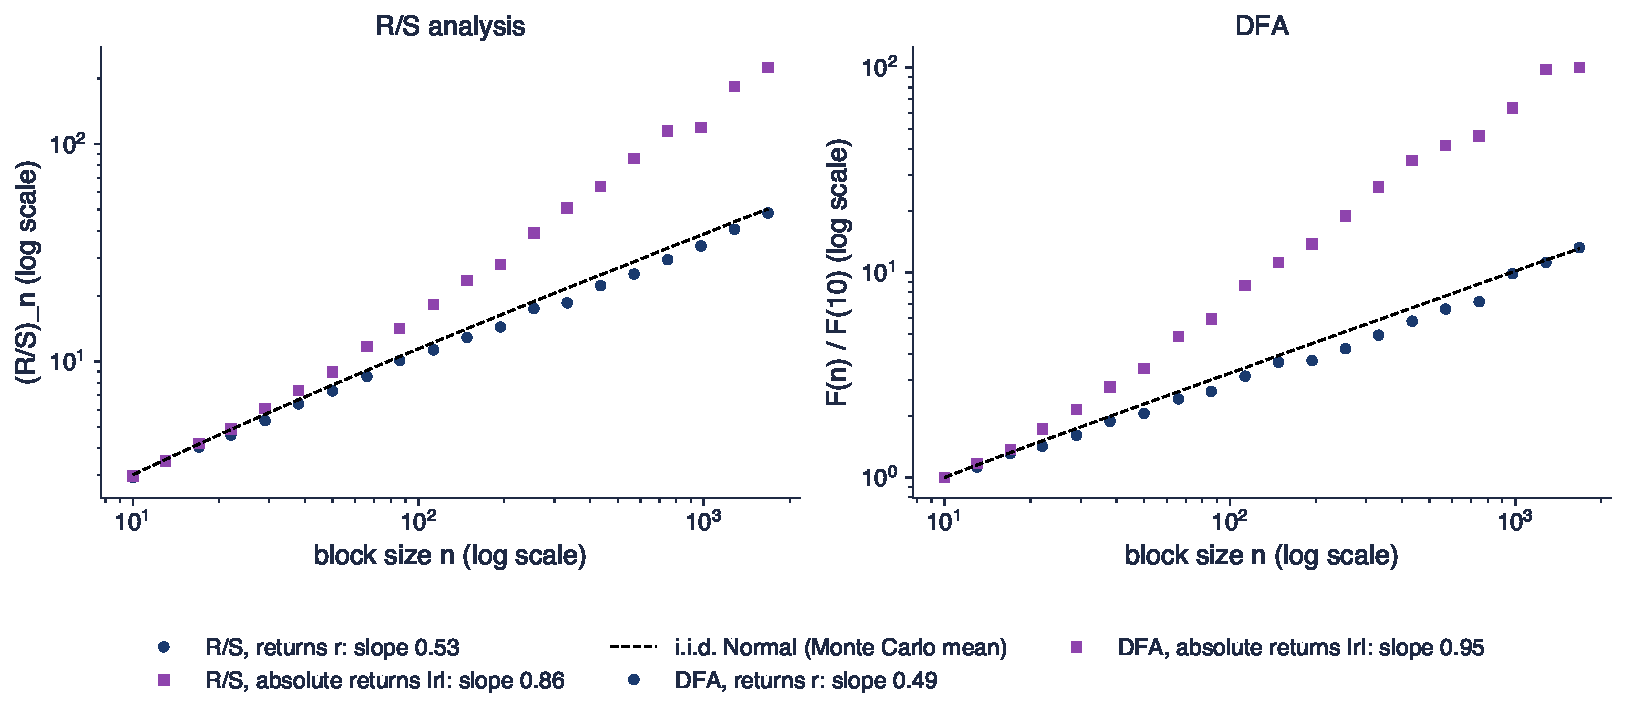
\includegraphics[width=0.97\textwidth,height=0.48\textheight,keepaspectratio]{sfm_ch11_rs_dfa.pdf}
\end{center}
\vspace{-0.25cm}
\begin{itemize}
    \item 20 de mărimi de bloc, de la 10 la 1678 de zile; linia întreruptă: curba medie a seriilor i.i.d.\ Normale de aceeași lungime
    \item Randamente: panta R/S $0{,}53$ (serii i.i.d.: $0{,}55$), DFA $0{,}49$ (i.i.d.: $0{,}50$): fără memorie lungă
    \item Randamente absolute: R/S $0{,}86$, DFA $0{,}95$: memorie lungă puternică a volatilității (secțiunea 7)
\end{itemize}
\sfmquantlet{Ch_11}{SFM_ch11_rs_estimators}
\end{frame}

\begin{frame}{Regresia GPH pe log-periodogramă}
\itemsize{\small}
\begin{itemize}
    \item \textbf{Periodograma} la frecvențele Fourier $\lambda_j = 2\pi j/T$: $I(\lambda_j) = \dfrac{1}{2\pi T}\left|\sum_{t=1}^{T} x_t e^{-i\lambda_j t}\right|^2$
    \begin{itemize}
        \item estimează densitatea spectrală, care se comportă ca $C\lambda^{-2d}$ lîngă zero
    \end{itemize}
    \item \textbf{GPH} \refGPH; \refFHH, 14.5.2: $\ln I(\lambda_j) = c - d\,\ln\!\left(4\sin^2(\lambda_j/2)\right) + e_j$, $j = 1, \dots, m$
    \begin{itemize}
        \item $\hat d$ = panta OLS în funcție de $-\ln(4\sin^2(\lambda_j/2))$; $\hat H = \hat d + 0{,}5$
        \item eroarea standard asimptotică $\pi/\sqrt{24m}$; lățimea de bandă $m = \lfloor T^{0{,}5}\rfloor$
    \end{itemize}
    \item Compromis: un $m$ mic păstrează doar frecvențele de termen lung (deplasare mică, varianță mare); un $m$ mare lasă să intre dinamica de termen scurt (deplasare)
\end{itemize}
\end{frame}

\begin{frame}{GPH: randamentele și randamentele absolute S\&P 500}
\itemsize{\footnotesize}
\begin{center}
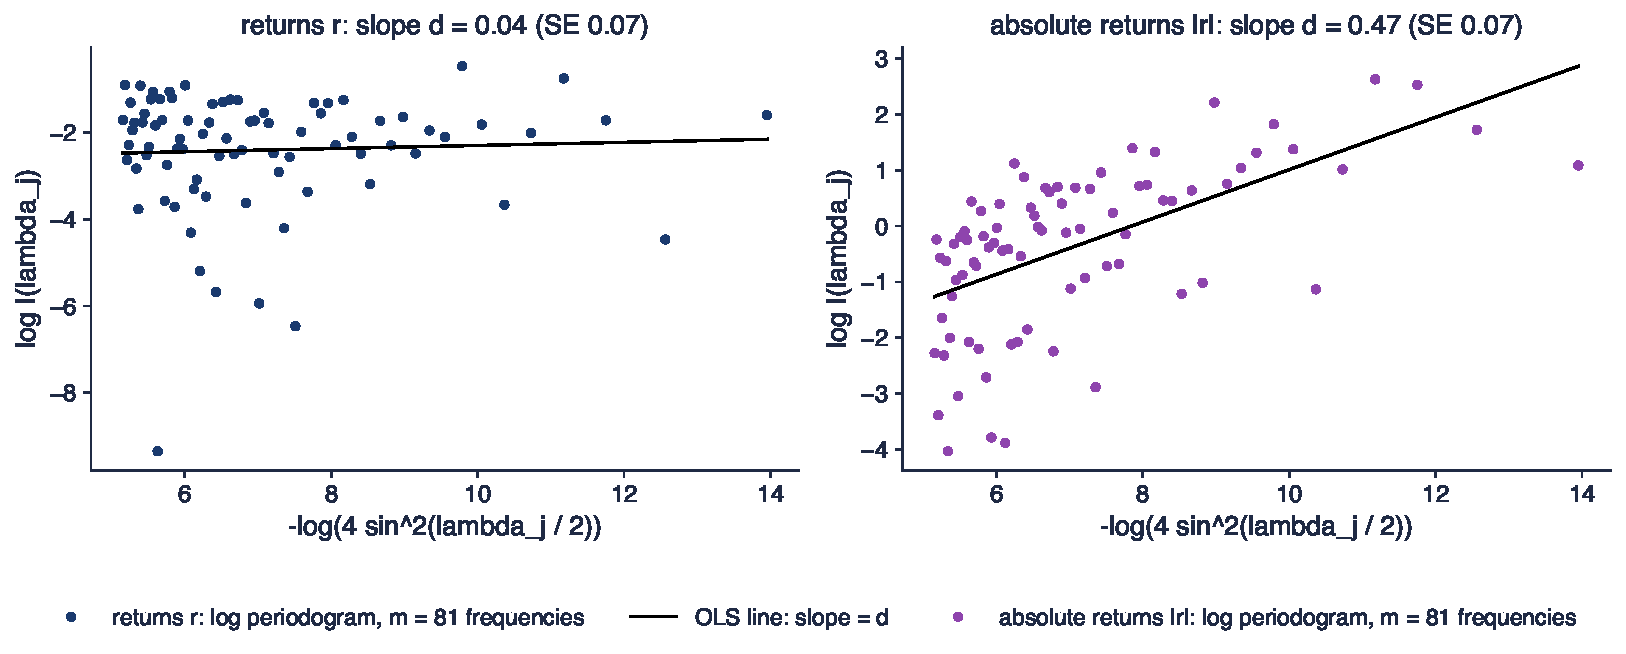
\includegraphics[width=0.97\textwidth,height=0.52\textheight,keepaspectratio]{sfm_ch11_gph.pdf}
\end{center}
\vspace{-0.25cm}
\begin{itemize}
    \item Se folosesc cele mai joase $m = 81$ frecvențe; fiecare punct este o frecvență
    \item Randamente: $\hat d = 0{,}036$ (SE $0{,}071$): nu diferă de 0; randamente absolute: $\hat d = 0{,}470$ (SE $0{,}071$), $\hat H = 0{,}97$
\end{itemize}
\sfmquantlet{Ch_11}{SFM_ch11_rs_estimators}
\end{frame}

\begin{frame}{Testul R/S modificat al lui Lo}
\itemsize{\footnotesize}
\begin{itemize}
    \item Problema: și memoria scurtă (de exemplu un AR(1)) mărește R/S, deci R/S clasic confundă memoria scurtă cu memoria lungă
    \item \refLo: $V_N(q) = \dfrac{R_N}{\sqrt{N}\,\hat\sigma_N(q)}$, $\hat\sigma^2_N(q) = \hat\gamma_0 + 2\sum_{j=1}^{q}\left(1 - \tfrac{j}{q + 1}\right)\hat\gamma_j$
    \begin{itemize}
        \item $\hat\gamma_j$: autocovarianțele de selecție; $\hat\sigma^2_N(q)$: varianța de lungă durată Newey--West \refNW; $q = 0$: R/S clasic
        \item $q = \lfloor (3N/2)^{1/3}\,(2\hat\rho_1/(1 - \hat\rho_1^2))^{2/3}\rfloor$, dependent de date (regula lui Andrews, folosită de Lo)
    \end{itemize}
    \item $H_0$: memorie scurtă; la 5\% respingem dacă $V_N(q) \notin [0{,}809, 1{,}862]$
    \begin{itemize}
        \item Concluzia lui Lo: nu există memorie lungă în randamentele indicilor bursieri din SUA, odată ce se ține cont de memoria scurtă
    \end{itemize}
\end{itemize}
\end{frame}

\begin{frame}{R/S clasic față de R/S modificat: mărimea și puterea testului}
\itemsize{\footnotesize}
\begin{center}
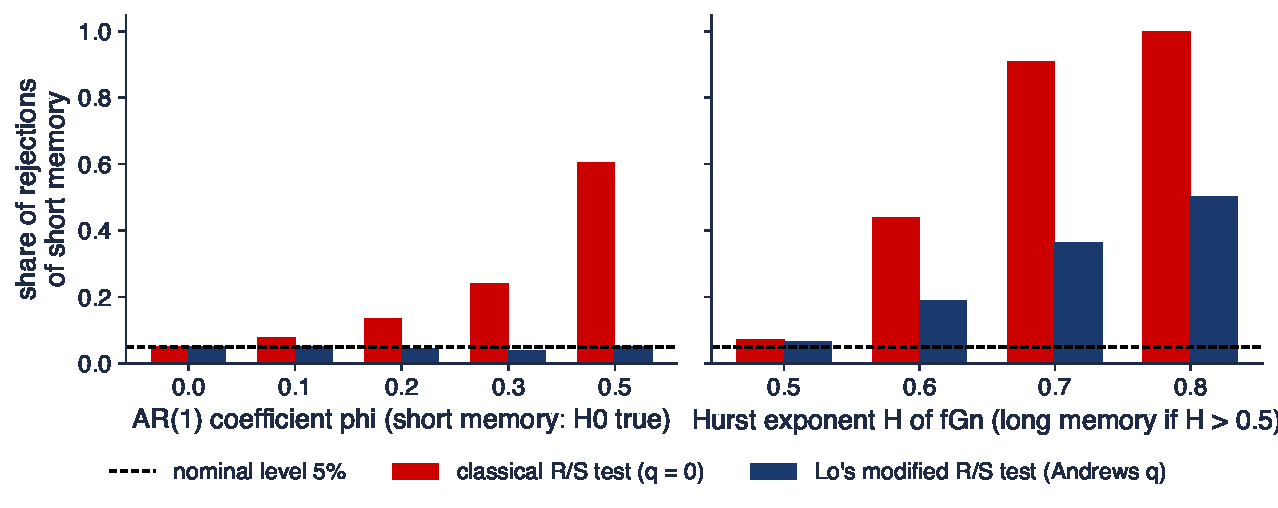
\includegraphics[width=0.97\textwidth,height=0.50\textheight,keepaspectratio]{sfm_ch11_lo_test.pdf}
\end{center}
\vspace{-0.25cm}
\begin{itemize}
    \item 500 de serii de 1000 de valori. Stînga, AR(1) (memorie scurtă, $H_0$ adevărată): pentru $\phi = 0{,}5$, testul clasic respinge în 60\% din cazuri, testul modificat în 5\%
    \item Dreapta, fGn (memorie lungă dacă $H > 0{,}5$): pentru $H = 0{,}7$, ratele de respingere sînt 91\% și 36\%: corecția costă putere \refTTW
\end{itemize}
\sfmquantlet{Ch_11}{SFM_ch11_monte_carlo}
\end{frame}

\begin{frame}{Eșantioane mici și benzi Monte Carlo}
\itemsize{\small}
\begin{itemize}
    \item Rezultatele asimptotice nu sînt de încredere pentru R/S și DFA la mărimile de eșantion din finanțe; folosim simularea \refWeron
    \begin{itemize}
        \item 1. simulăm multe serii i.i.d.\ Normale, de aceeași lungime $N$ ca datele
        \item 2. aplicăm exact același estimator (aceleași mărimi de bloc, aceeași lățime de bandă)
        \item 3. cuantilele de 2,5\% și 97,5\% ale lui $\hat H$ formează banda de 95\% sub $H = 0{,}5$
    \end{itemize}
    \item Respingem $H = 0{,}5$ doar dacă $\hat H$ se află în afara benzii
    \item Seria i.i.d.\ Normală este cea mai simplă ipoteză nulă; un model estimat cu memorie scurtă (AR, GARCH) dă o ipoteză nulă mai exigentă (secțiunea 6)
\end{itemize}
\end{frame}

\begin{frame}{Monte Carlo: deplasarea și dispersia estimatorilor}
\itemsize{\footnotesize}
\begin{center}
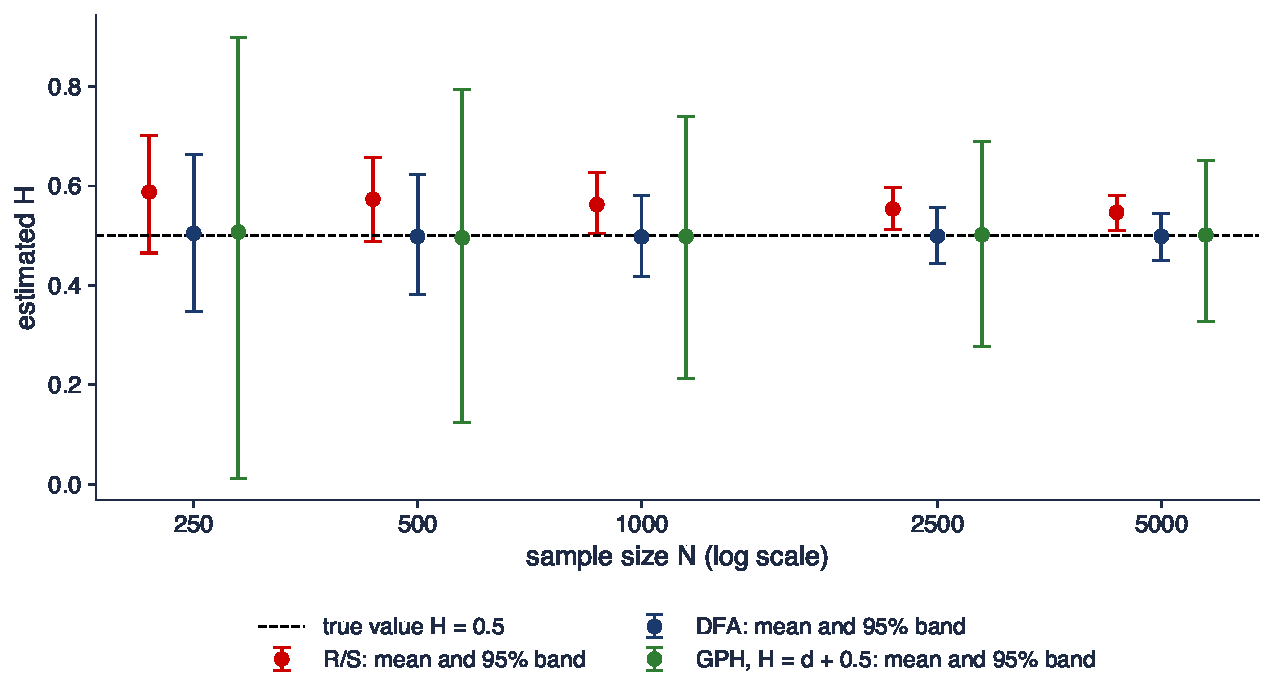
\includegraphics[width=0.97\textwidth,height=0.50\textheight,keepaspectratio]{sfm_ch11_mc_bias.pdf}
\end{center}
\vspace{-0.25cm}
\begin{itemize}
    \item 500 de serii i.i.d.\ Normale pentru fiecare $N$; valoarea adevărată este $H = 0{,}5$
    \item R/S: media $0{,}562$ la $N = 1000$ (deplasată în sus); DFA: $0{,}497$; GPH: $0{,}498$, nedeplasat, dar cu dispersie mare
    \item Lățimea benzii de 95\% la $N = 1000$: R/S $0{,}12$, DFA $0{,}16$, GPH $0{,}53$; la $N = 250$: DFA $0{,}32$
\end{itemize}
\sfmquantlet{Ch_11}{SFM_ch11_monte_carlo}
\end{frame}

\begin{frame}{S\&P 500: toți estimatorii}
\itemsize{\small}
\begin{center}
\footnotesize
\begin{tabular}{lrrrrr}
\toprule
 & R/S & DFA & GPH $\hat d$ (SE) & Lo $V_N(q)$ & $q$ \\
\midrule
randamente $r_t$ & $0{,}53$ & $0{,}49$ & $0{,}04$ ($0{,}07$) & $1{,}56$ & 7 \\
randamente absolute $|r_t|$ & $0{,}86$ & $0{,}95$ & $0{,}47$ ($0{,}07$) & $2{,}66$ & 15 \\
banda de 95\%, i.i.d. & $[0{,}51; 0{,}57]$ & $[0{,}46; 0{,}54]$ & $[0{,}36; 0{,}65]$ & $[0{,}809, 1{,}862]$ &  \\
\bottomrule
\end{tabular}
\end{center}
\begin{itemize}
    \item $N = 6\,714$ randamente zilnice, din 2000 pînă la 18 septembrie 2026; banda GPH este dată pentru $\hat H = \hat d + 0{,}5$
    \item Randamente: fiecare estimare se află în banda ei, $V_N(q)$ se află în $[0{,}809, 1{,}862]$
    \item Randamente absolute: fiecare estimare este mult peste banda ei, iar testul lui Lo respinge memoria scurtă
\end{itemize}
\end{frame}

\begin{frame}{Interpretarea rezultatelor: S\&P 500}
\itemsize{\small}
\begin{itemize}
    \item Direcția randamentelor nu are memorie lungă din 2000 încoace
    \begin{itemize}
        \item în acord cu forma slabă a EMH (\sfmchlink{https://danpele.github.io/SFM/RO/Cursuri/capitol7_piete_eficiente_mers_aleator_vr.pdf}{Capitolul 7}) și cu \refLo
        \item doar R/S ($0{,}53$) ar părea să indice „$H > 0{,}5$”; banda lui începe de la $0{,}51$
    \end{itemize}
    \item Mărimea randamentelor are memorie lungă: $\hat d = 0{,}47$ pentru $|r_t|$
    \begin{itemize}
        \item riscul unei perioade liniștite sau agitate persistă luni de zile: versiunea pe termen lung a volatility clustering
    \end{itemize}
    \item Înainte de a concluziona că există memorie lungă, eliminăm memoria lungă aparentă: secțiunea următoare
\end{itemize}
\end{frame}

\begin{frame}{Recapitulare: estimatori ai memoriei lungi}
\itemsize{\small}
\begin{itemize}
    \item R/S și DFA: pantele unor grafice log-log; GPH: panta unei regresii pe log-periodogramă
    \item R/S modificat al lui Lo corectează efectul memoriei scurte, dar pierde putere
    \item Evaluăm fiecare estimare față de o bandă Monte Carlo pentru același $N$
\end{itemize}
\end{frame}


%=============================================================================
\section{Memorie lungă aparentă}
%=============================================================================

\begin{frame}{Rupturile structurale par memorie}
\itemsize{\small}
\begin{itemize}
    \item O serie cu cîteva schimbări ale mediei are o ACF de selecție care scade lent, ca la memoria lungă
    \begin{itemize}
        \item două regimuri cu mediile $\mu_1 \neq \mu_2$: orice pereche de observații din același regim are în comun abaterea $\mu_i - \bar x$
    \end{itemize}
    \item Rezultate de referință
    \begin{itemize}
        \item \refDI: schimbările rare de regim produc estimări ale lui $d$ care nu se pot deosebi de memoria lungă reală
        \item \refGH: o parte din memoria lungă a randamentelor absolute S\&P 500 provine din rupturi ocazionale
        \item \refLS: memoria lungă a pătratelor randamentelor S\&P 500 rezistă verificărilor; în randamente nu apare
    \end{itemize}
    \item Teste ale memoriei lungi reale față de cea aparentă: \refFHH, 14.4.3
\end{itemize}
\end{frame}

\begin{frame}{Nilul în 1898: o ruptură, nu doar memorie}
\itemsize{\footnotesize}
\begin{columns}[T]
\begin{column}{0.55\textwidth}
\begin{itemize}
    \item \refCobb: debitul anual al Nilului la Aswan, 1871--1970, își schimbă media după 1898
    \item Debitul mediu: 1098 înainte, 850 după (în $10^8$ m$^3$), o scădere de 23\%
    \item Schimbarea coincide cu construcția barajului Aswan Low Dam (1898--1902)
    \item O serie hidrologică cu o ruptură ridică aceeași problemă ca o piață care își schimbă regimul
\end{itemize}
\end{column}
\begin{column}{0.41\textwidth}
\centering
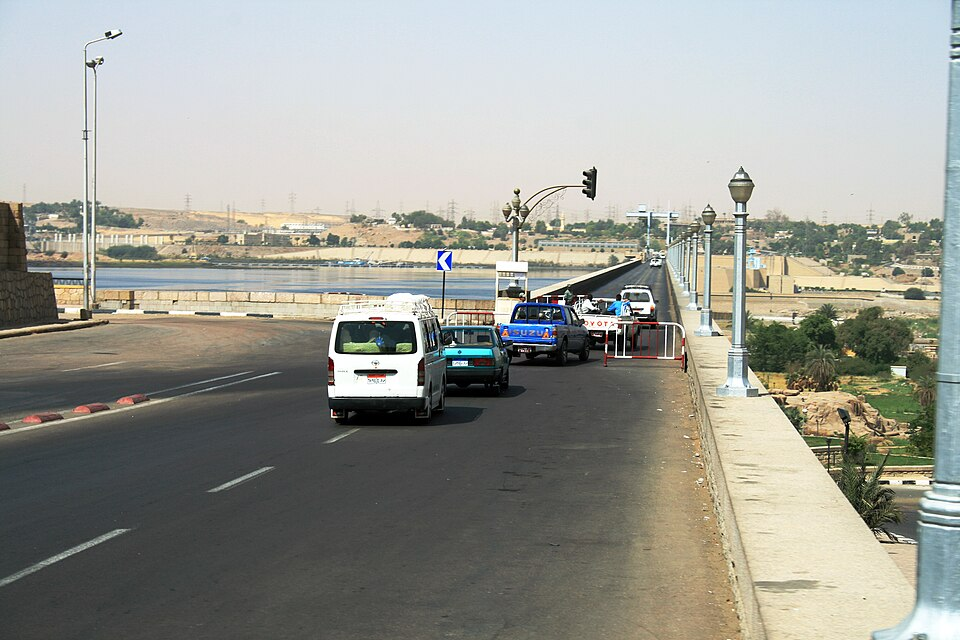
\includegraphics[height=0.36\textheight]{ch11_aswan_low_dam.jpg}\\[1mm]
\imgcap{Barajul Aswan Low Dam de pe Nil}
\imgcredit{https://commons.wikimedia.org/wiki/File:Aswan_Low_Dam_Egypt_1.jpg}{Foto: Karelj (2010); domeniu public; Wikimedia Commons}
\end{column}
\end{columns}
\end{frame}

\begin{frame}{Nilul: R/S înainte și după eliminarea rupturii}
\itemsize{\footnotesize}
\begin{center}
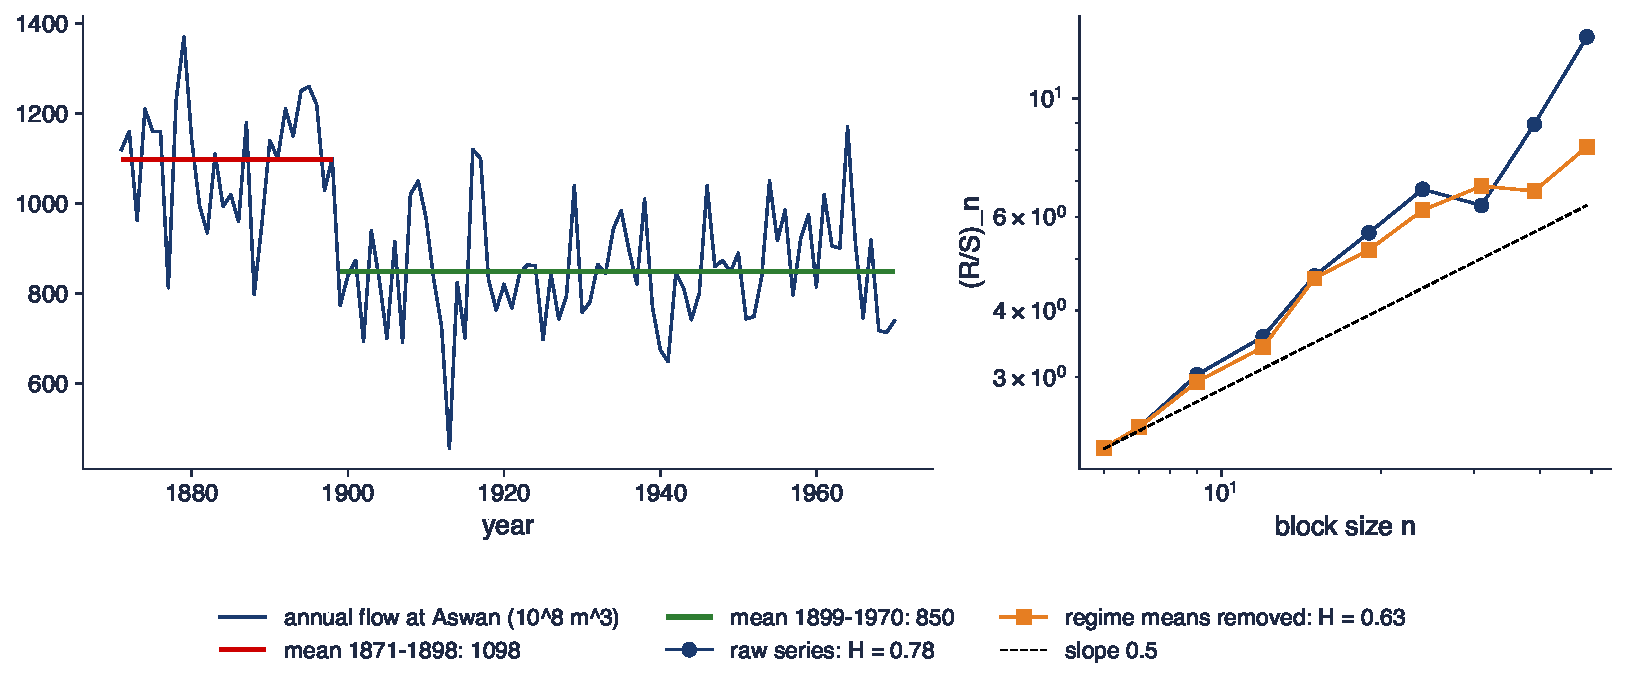
\includegraphics[width=0.97\textwidth,height=0.50\textheight,keepaspectratio]{sfm_ch11_nile.pdf}
\end{center}
\vspace{-0.25cm}
\begin{itemize}
    \item Seria brută: $\hat H_{R/S} = 0{,}78$, DFA $0{,}84$; după eliminarea celor două medii de regim: $0{,}63$ și $0{,}50$
    \item Cu $N = 100$, banda i.i.d.\ pentru R/S este largă, $[0{,}45; 0{,}75]$, centrată în $0{,}60$: cea mai mare parte a memoriei aparente era ruptura
\end{itemize}
\sfmquantlet{Ch_11}{SFM_ch11_spurious}
\end{frame}

\begin{frame}{Memorie lungă aparentă în simulări}
\itemsize{\footnotesize}
\begin{center}
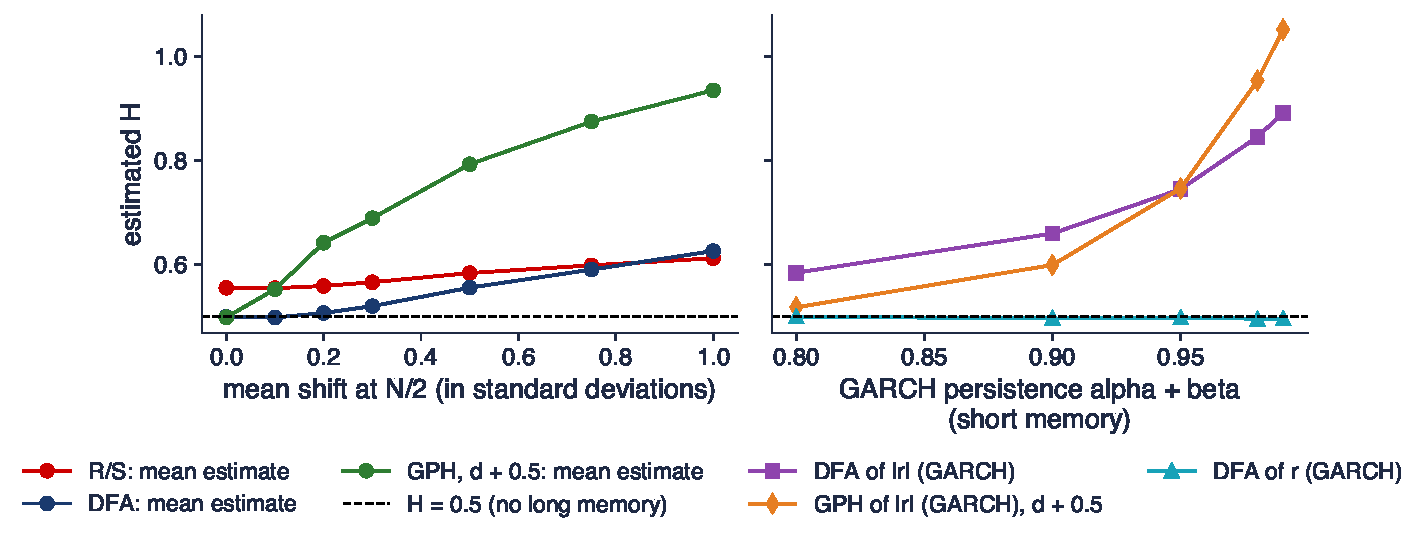
\includegraphics[width=0.97\textwidth,height=0.48\textheight,keepaspectratio]{sfm_ch11_spurious.pdf}
\end{center}
\vspace{-0.25cm}
\begin{itemize}
    \item 300 de serii de 2000 de valori. Stînga: i.i.d.\ $N(0,1)$ cu o schimbare a mediei la mijloc; o schimbare de 0,5 abateri standard dă GPH $\hat H = 0{,}79$, DFA $0{,}56$
    \item Dreapta: GARCH(1,1), un model cu memorie scurtă (\sfmchlink{https://danpele.github.io/SFM/RO/Cursuri/capitol9_modele_arch_garch.pdf}{Capitolul 9}); pentru $|r_t|$, DFA dă $0{,}74$ la $\alpha + \beta = 0{,}95$ și $0{,}89$ la $0{,}99$; randamentele rămîn la $0{,}50$
\end{itemize}
\sfmquantlet{Ch_11}{SFM_ch11_spurious}
\end{frame}

\begin{frame}{Volatility clustering imită memoria lungă}
\itemsize{\small}
\begin{itemize}
    \item În GARCH(1,1), ACF a lui $r_t^2$ scade ca $(\alpha + \beta)^k$: memorie scurtă
    \begin{itemize}
        \item cu $\alpha + \beta$ apropiat de 1, scăderea este atît de lentă încît un eșantion de cîteva mii de zile nu o poate deosebi de $k^{2d - 1}$
    \end{itemize}
    \item Consecință: un $\hat H$ mare pentru $|r_t|$ este compatibil cu un GARCH persistent; nu este, singur, o dovadă de dinamică fracționară
    \item Pentru randamente, GARCH nu creează memorie: estimările rămîn la 0,5 (panoul din dreapta)
    \item O ipoteză nulă mai bună: simulăm GARCH-ul estimat și comparăm $\hat H$ al datelor cu banda GARCH
\end{itemize}
\end{frame}

\begin{frame}{Verificări împotriva memoriei lungi aparente}
\itemsize{\small}
\begin{itemize}
    \item \textbf{Testul permutării}: permutăm aleator seria; distribuția rămîne, ordinea dispare; $\hat H$ ar trebui să scadă la 0,5
    \item \textbf{Subeșantioane}: estimăm înainte și după rupturile cunoscute (2008, 2020); memoria lungă reală apare în fiecare subeșantion
    \item \textbf{Mai mulți estimatori și lățimi de bandă}: R/S, DFA, GPH cu $m = T^{0{,}5}$ și $T^{0{,}6}$ ar trebui să concorde
    \item \textbf{R/S modificat al lui Lo}: elimină efectul memoriei scurte
    \item \textbf{Ipoteză nulă pe baza unui model}: benzi Monte Carlo dintr-un AR sau GARCH estimat, în locul zgomotului i.i.d.
\end{itemize}
\end{frame}

\begin{frame}{Recapitulare: memorie lungă aparentă}
\itemsize{\small}
\begin{itemize}
    \item Schimbările mediei și ale regimului produc ACF de selecție care scad lent
    \item Volatilitatea GARCH persistentă arată ca memoria lungă în $|r_t|$ în eșantioane finite
    \item Permutăm, împărțim eșantionul, comparăm estimatorii, folosim o ipoteză nulă pe baza unui model
\end{itemize}
\end{frame}


%=============================================================================
\section{Memoria lungă a volatilității}
%=============================================================================

\begin{frame}{S\&P 500: ACF pentru $r_t$, $|r_t|$ și $r_t^2$}
\itemsize{\footnotesize}
\begin{center}
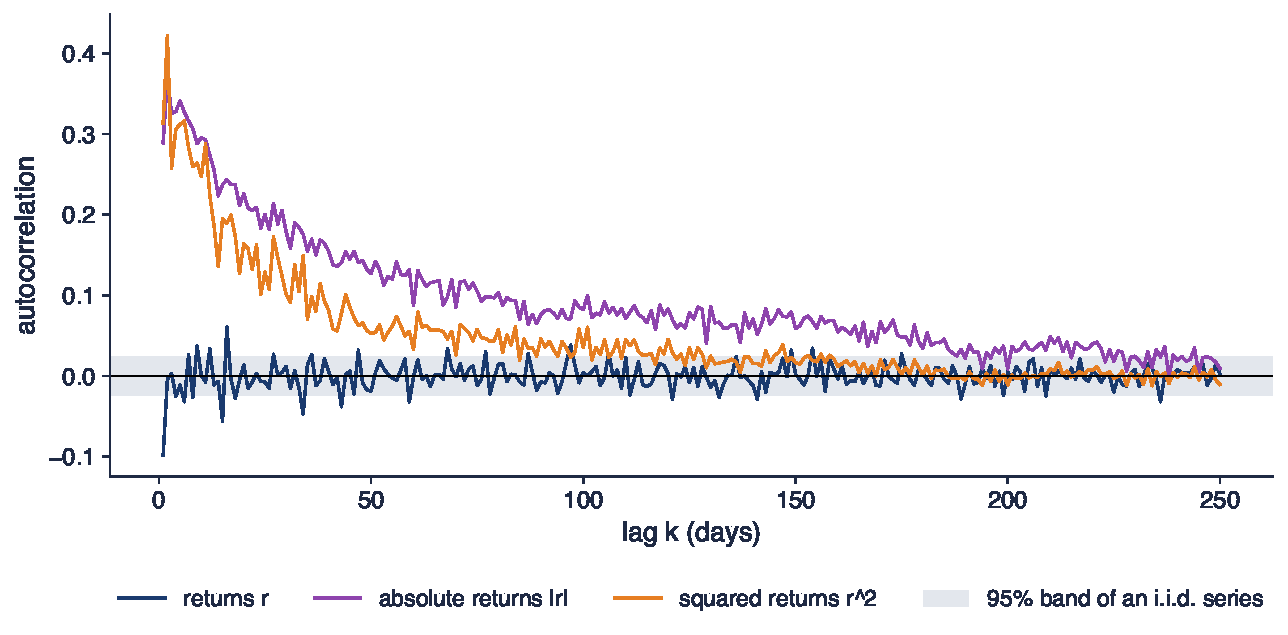
\includegraphics[width=0.97\textwidth,height=0.48\textheight,keepaspectratio]{sfm_ch11_vol_acf.pdf}
\end{center}
\vspace{-0.25cm}
\begin{itemize}
    \item $|r_t|$: $\rho(1) = 0{,}289$, $\rho(50) = 0{,}127$, $\rho(100) = 0{,}082$; 227 dintre primele 250 de decalaje sînt peste banda $0{,}024$
    \item $r_t^2$: $\rho(1) = 0{,}313$, $\rho(50) = 0{,}053$; $r_t$: $\rho(1) = -0{,}099$, apoi în interiorul benzii
    \item \refDGE: $|r_t|$ este mai persistent decît $r_t^2$, care este mai afectat de zilele extreme izolate
\end{itemize}
\sfmquantlet{Ch_11}{SFM_ch11_volatility_memory}
\end{frame}

\begin{frame}{Șase piețe: randamente și randamente absolute}
\itemsize{\footnotesize}
\begin{center}
\scriptsize
\begin{tabular}{lrrrrrrrr}
\toprule
 & $N$ & \multicolumn{3}{c}{randamente $r_t$} & \multicolumn{3}{c}{randamente absolute $|r_t|$} & banda DFA \\
 & & R/S & DFA & GPH $\hat d$ & DFA & GPH $\hat d$ & Lo $V$ &  \\
\midrule
S\&P 500 & 6\,714 & $0{,}53$ & $0{,}49$ & $0{,}04$ & $0{,}95$ & $0{,}47$ & $2{,}66$ & $[0{,}46; 0{,}54]$ \\
DAX & 6\,786 & $0{,}55$ & $0{,}50$ & $-0{,}06$ & $0{,}94$ & $0{,}48$ & $3{,}43$ & $[0{,}45; 0{,}54]$ \\
BET & 6\,670 & $0{,}58$ & $0{,}57$ & $0{,}17$ & $0{,}85$ & $0{,}47$ & $4{,}47$ & $[0{,}45; 0{,}54]$ \\
Bitcoin & 4\,384 & $0{,}59$ & $0{,}56$ & $0{,}05$ & $0{,}82$ & $0{,}33$ & $3{,}94$ & $[0{,}45; 0{,}55]$ \\
TLV & 3\,788 & $0{,}54$ & $0{,}47$ & $-0{,}06$ & $0{,}76$ & $0{,}25$ & $2{,}47$ & $[0{,}45; 0{,}55]$ \\
SNP & 3\,815 & $0{,}55$ & $0{,}49$ & $-0{,}02$ & $0{,}73$ & $0{,}21$ & $2{,}39$ & $[0{,}45; 0{,}55]$ \\
\bottomrule
\end{tabular}
\end{center}
\begin{itemize}
    \item Date zilnice pînă la 18 septembrie 2026: S\&P 500, DAX, BET din 2000, Bitcoin din 2014, TLV și SNP din 2010; eroarea standard GPH este de circa $0{,}07$--$0{,}08$
    \item Randamentele BET: DFA $0{,}57$ peste banda sa, GPH $\hat d = 0{,}17$, testul lui Lo ($V = 1{,}96$) respinge memoria scurtă
    \item Randamente absolute: $\hat d$ între $0{,}21$ și $0{,}48$; testul lui Lo respinge pentru toate cele șase serii
\end{itemize}
\end{frame}

\begin{frame}{Șase piețe: exponenții DFA și testul permutării}
\itemsize{\footnotesize}
\begin{center}
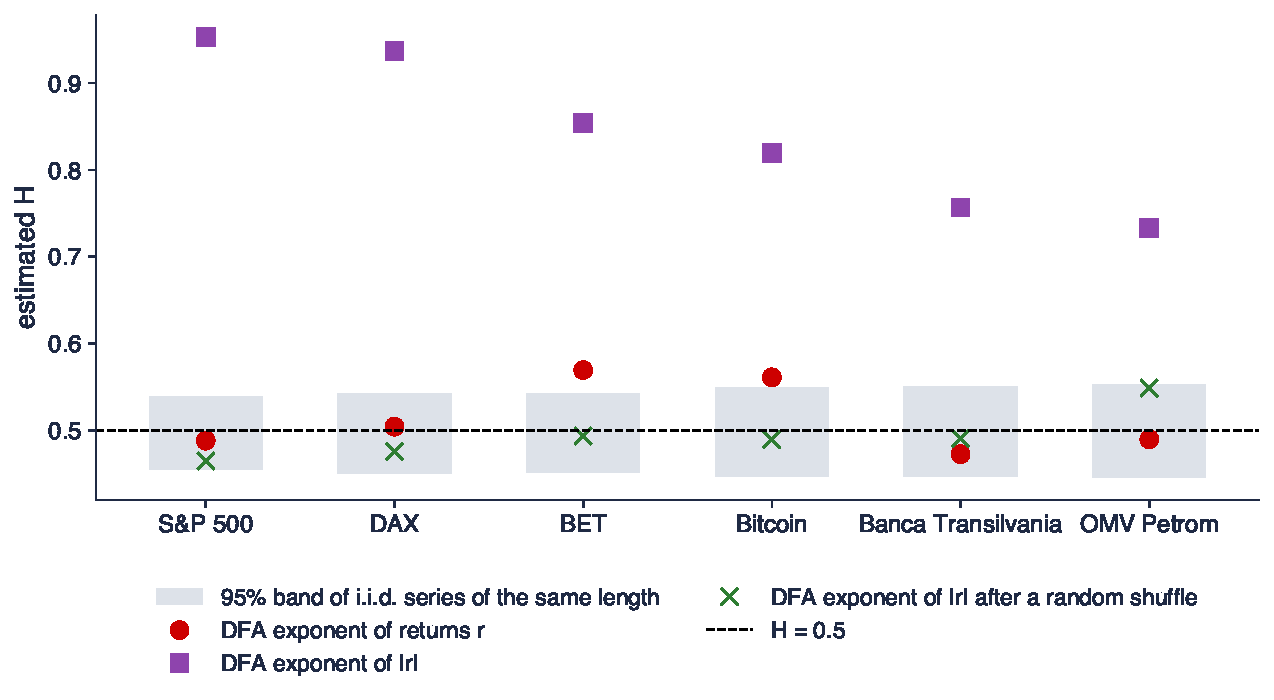
\includegraphics[width=0.97\textwidth,height=0.50\textheight,keepaspectratio]{sfm_ch11_markets.pdf}
\end{center}
\vspace{-0.25cm}
\begin{itemize}
    \item Zona colorată: banda de 95\% a seriilor i.i.d.\ de aceeași lungime; cercuri: randamente; pătrate: $|r_t|$; cruciulițe: $|r_t|$ după o permutare aleatoare
    \item $|r_t|$: DFA între $0{,}73$ și $0{,}95$; după permutare: între $0{,}46$ și $0{,}55$, în interiorul benzilor: memoria se află în ordinea zilelor
\end{itemize}
\sfmquantlet{Ch_11}{SFM_ch11_volatility_memory}
\end{frame}

\begin{frame}{Interpretarea rezultatelor: ce este previzibil?}
\itemsize{\small}
\begin{itemize}
    \item \textbf{Randamentele}: fără memorie lungă la S\&P 500, DAX, TLV și SNP; Bitcoin la limita benzii
    \begin{itemize}
        \item BET: persistență, ca în testele raportului varianțelor din \sfmchlink{https://danpele.github.io/SFM/RO/Cursuri/capitol7_piete_eficiente_mers_aleator_vr.pdf}{Capitolul 7}; în parte, efectul tranzacționării reduse din primii ani (secțiunea 8)
    \end{itemize}
    \item \textbf{Volatilitatea}: memorie lungă peste tot, cea mai puternică la marii indici de acțiuni
    \begin{itemize}
        \item regimul de risc de azi este informativ luni de zile: util pentru VaR (value at risk, valoarea expusă la risc) și pentru evaluarea opțiunilor
    \end{itemize}
    \item Eficiența în formă slabă (direcție imprevizibilă) și riscul previzibil coexistă: FMH adaugă o explicație, investitorii cu orizonturi diferite reacționează la volatilitate pe scale de timp diferite
\end{itemize}
\end{frame}

\begin{frame}{Modele pentru memoria lungă a volatilității}
\itemsize{\small}
\begin{itemize}
    \item \textbf{FIGARCH} (fractionally integrated GARCH, GARCH fracționar integrat) \refBBM; \refFHH, 14.6.2: $(1 - L)^d$ aplicat lui $\varepsilon_t^2$
    \begin{itemize}
        \item șocurile de volatilitate scad hiperbolic; $d = 0$ dă GARCH, $d = 1$ dă IGARCH (integrated GARCH, GARCH integrat, \sfmchlink{https://danpele.github.io/SFM/RO/Cursuri/capitol9_modele_arch_garch.pdf}{Capitolul 9})
    \end{itemize}
    \item \textbf{Orizonturi eterogene}, ideea FMH în modelele de volatilitate
    \begin{itemize}
        \item \refMuller: componente ale pieței cu rezoluții de timp diferite (de la traderii intraday la investitorii pe termen lung)
        \item \refAB: multe componente de volatilitate cu persistențe diferite se însumează și dau memorie lungă
        \item \refCorsi: modelul HAR (heterogeneous autoregressive, autoregresiv heterogen), volatilitatea de mîine în funcție de volatilitatea zilnică, săptămînală și lunară: trei orizonturi, memorie lungă aproximativă
    \end{itemize}
\end{itemize}
\end{frame}

\begin{frame}{Recapitulare: memoria lungă a volatilității}
\itemsize{\small}
\begin{itemize}
    \item $|r_t|$ și $r_t^2$: ACF cu scădere hiperbolică, $\hat d$ în jur de 0,2--0,5 pe toate cele șase piețe
    \item Randamentele: fără memorie lungă, cu excepția BET
    \item FIGARCH și HAR o modelează; HAR este o traducere directă a orizonturilor eterogene
\end{itemize}
\end{frame}


%=============================================================================
\section{Exponenți Hurst pe ferestre mobile}
%=============================================================================

\begin{frame}{Se schimbă eficiența în timp?}
\itemsize{\small}
\begin{itemize}
    \item AMH și FMH prezic, amîndouă, că memoria pieței se schimbă în timp
    \begin{itemize}
        \item \refCT: exponenți Hurst pe ferestre mobile pentru piețe emergente, pentru a testa dacă devin mai eficiente
        \item \refBar: DFA pe ferestre mobile pentru randamentele și volatilitatea Bitcoin
    \end{itemize}
    \item Abordarea folosită aici
    \begin{itemize}
        \item ferestre de 1000 de observații (circa patru ani de zile de tranzacționare), mutate cu 21 de observații (circa o lună)
        \item DFA pe $r_t$ și pe $|r_t|$; fiecare estimare este datată la ultima zi a ferestrei, deci folosește doar date trecute
        \item banda Monte Carlo de 95\% pentru $N = 1000$: $[0{,}42; 0{,}58]$
    \end{itemize}
\end{itemize}
\end{frame}

\begin{frame}{Exponenți DFA pe ferestre mobile: S\&P 500, BET, Bitcoin}
\itemsize{\footnotesize}
\begin{center}
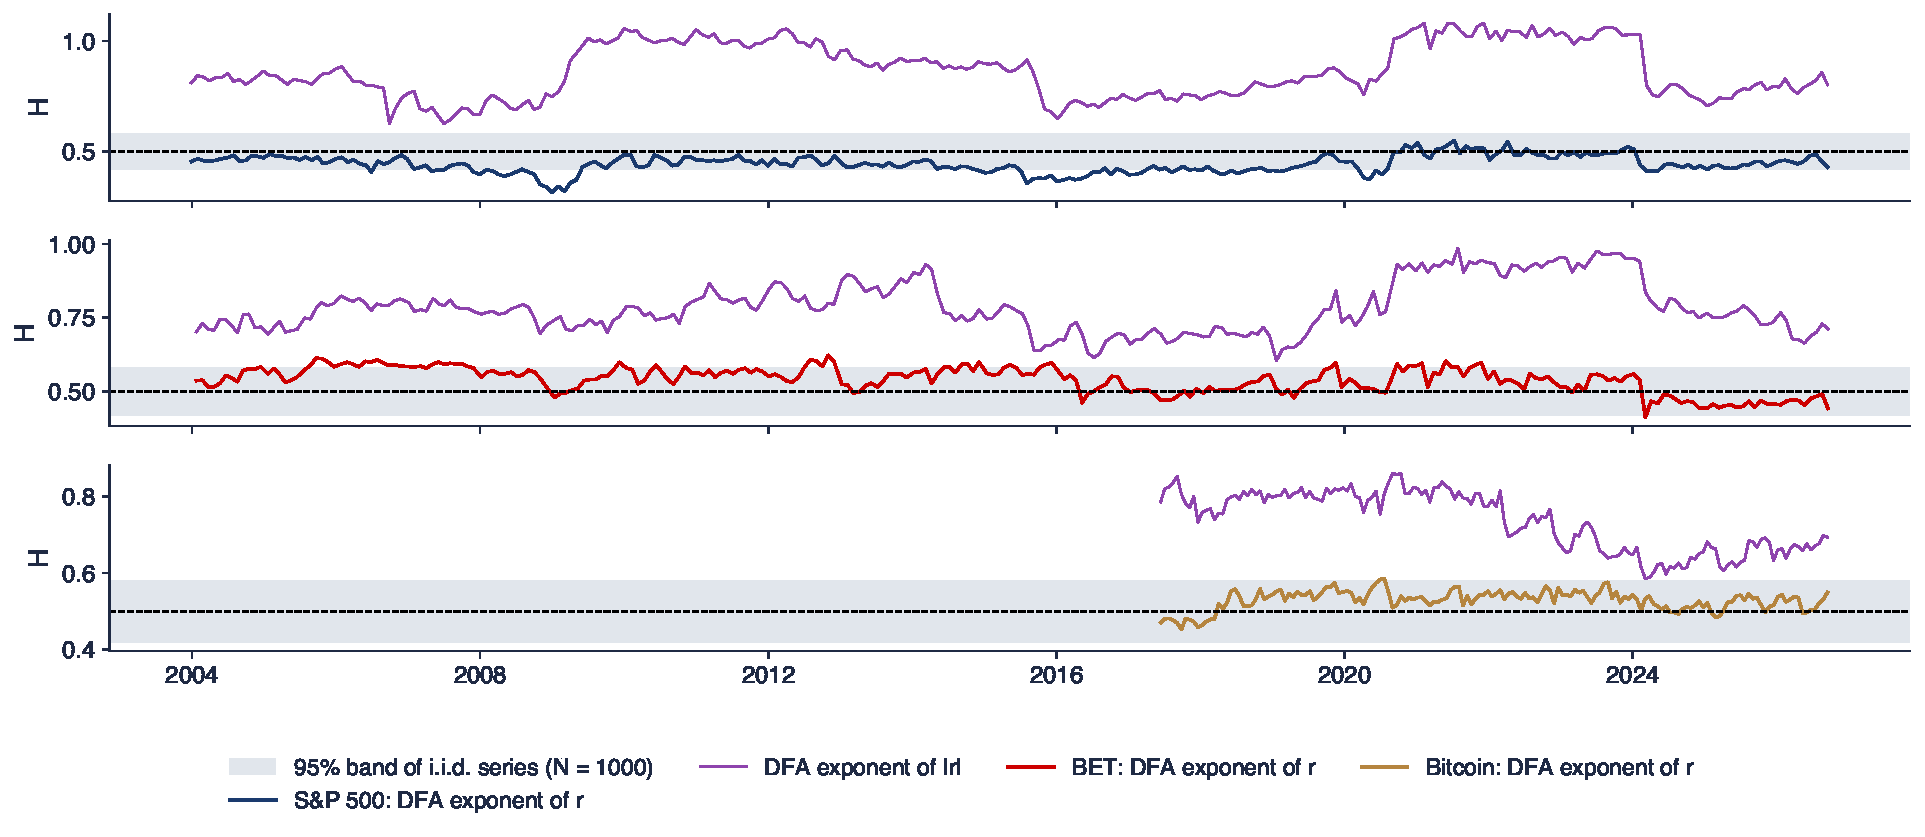
\includegraphics[width=0.97\textwidth,height=0.60\textheight,keepaspectratio]{sfm_ch11_rolling.pdf}
\end{center}
\vspace{-0.25cm}
\begin{itemize}
    \item De sus în jos: S\&P 500, BET, Bitcoin; linia colorată: $r_t$; linia mov: $|r_t|$; zona colorată: banda i.i.d.
    \item $|r_t|$ mereu mult peste bandă; exponentul lui crește în timpul și după crize (2008--2009, 2020)
\end{itemize}
\sfmquantlet{Ch_11}{SFM_ch11_rolling_hurst}
\end{frame}

\begin{frame}{Interpretarea exponenților pe ferestre mobile}
\itemsize{\small}
\begin{itemize}
    \item S\&P 500: 273 de ferestre; $\hat H$ al randamentelor între $0{,}32$ și $0{,}55$; 24\% dintre ferestre sub bandă, niciuna peste
    \begin{itemize}
        \item minimul, la 31 decembrie 2008, vine după crahul din 2008: inversări zilnice (antipersistență) în panică
    \end{itemize}
    \item BET: 20\% dintre ferestre peste bandă; $\hat H$ mediu $0{,}56$ în prima treime a ferestrelor, $0{,}52$ în ultima treime
    \begin{itemize}
        \item maximul este atins la 31 octombrie 2012; apoi piața devine mai eficientă, pe măsură ce lichiditatea crește
    \end{itemize}
    \item Bitcoin: ferestre din 13 iunie 2017; $\hat H$ între $0{,}45$ și $0{,}59$, 1\% dintre ferestre peste bandă
\end{itemize}
\end{frame}

\begin{frame}{Studiu de caz: este Bitcoin eficient?}
\itemsize{\footnotesize}
\begin{columns}[T]
\begin{column}{0.60\textwidth}
\begin{itemize}
    \item \refUrq: mai multe teste, printre care R/S, pe Bitcoin, 2010--2016
    \begin{itemize}
        \item ineficient pe întregul eșantion, cu o evoluție spre eficiență în ultimii ani
    \end{itemize}
    \item \refNC: aceleași date după o transformare de tip putere a randamentelor: în acord cu eficiența în formă slabă
    \item \refBar: DFA pe ferestre mobile: randamente persistente pînă în 2014, apropiate de $H = 0{,}5$ după aceea; memorie lungă a volatilității pe toată perioada
    \item Ferestrele noastre încep în 2017 și confirmă: randamente lîngă bandă, $|r_t|$ mult peste ea
\end{itemize}
\end{column}
\begin{column}{0.36\textwidth}
\centering
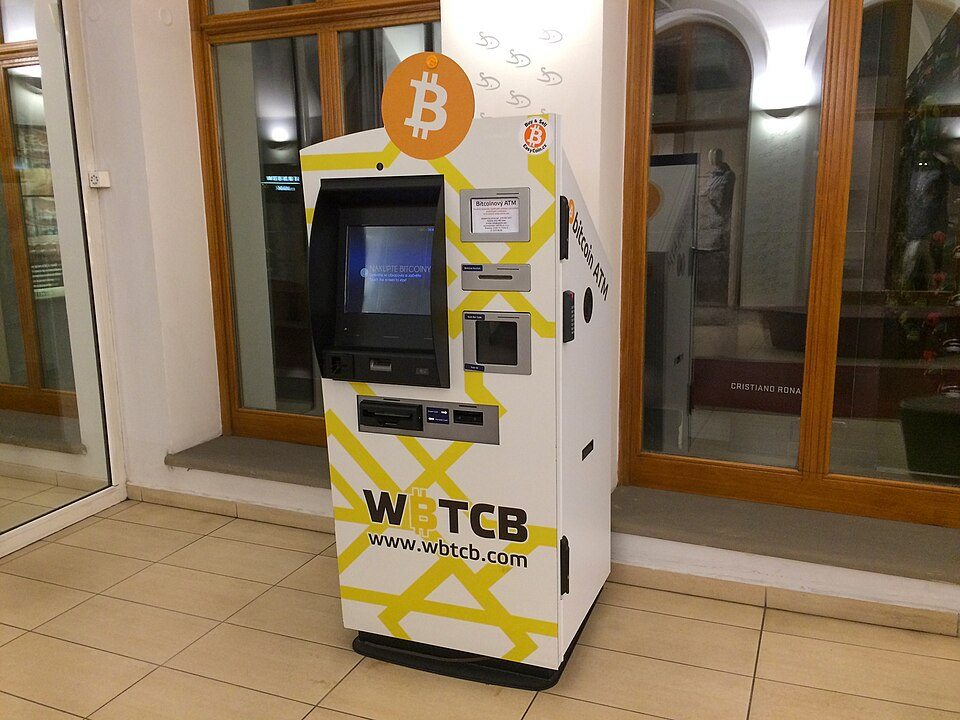
\includegraphics[height=0.40\textheight]{ch11_bitcoin_atm_prague.jpg}\\[1mm]
\imgcap{Un bancomat Bitcoin la Praga (2016)}
\imgcredit{https://commons.wikimedia.org/wiki/File:Bitcoin_ATM_Prague.jpg}{Foto: Perituss (2016); CC0; Wikimedia Commons}
\end{column}
\end{columns}
\end{frame}

\begin{frame}{Capcanele estimărilor pe ferestre mobile}
\itemsize{\small}
\begin{itemize}
    \item \textbf{Testarea multiplă}: 273 de ferestre, fiecare la 5\%, dau din întîmplare circa 14 ferestre în afara benzii
    \begin{itemize}
        \item căutăm perioade lungi în afara benzii, nu ferestre izolate
    \end{itemize}
    \item \textbf{Suprapunerea}: ferestrele consecutive au în comun 979 dintre cele 1000 de observații; traiectoria este netedă prin construcție
    \item \textbf{Lungimea ferestrei}: ferestrele mai scurte reacționează mai repede, dar au benzi mai largi (DFA, $N = 250$: lățimea $0{,}32$)
    \item \textbf{Regimurile de volatilitate}: o criză din interiorul unei ferestre deplasează estimarea timp de patru ani
    \item \textbf{Datarea}: datăm fiecare estimare la sfîrșitul ferestrei, niciodată la mijloc (fără informație din viitor)
\end{itemize}
\end{frame}

\begin{frame}{Recapitulare: exponenți Hurst pe ferestre mobile}
\itemsize{\small}
\begin{itemize}
    \item $\hat H$ pe ferestre mobile, cu o bandă Monte Carlo, arată cum se schimbă memoria în timp
    \item BET: persistent la început, mai aproape de 0,5 ulterior; S\&P 500: niciodată persistent; Bitcoin: aproape de 0,5 din 2017
    \item Interpretăm perioade, nu ferestre izolate; datăm la sfîrșitul ferestrei
\end{itemize}
\end{frame}


%=============================================================================
\section{Memoria lungă și riscul}
%=============================================================================

\begin{frame}{Scalarea riscului cu $h^H$}
\itemsize{\footnotesize}
\begin{itemize}
    \item Dacă randamentele sînt autosimilare: VaR 1\% pe $h$ zile $= z_{0{,}99}\,\sigma\,h^H$, cu $z_{0{,}99} = 2{,}326$ (cazul Normal)
    \begin{itemize}
        \item volatilitatea zilnică $\sigma = 1{,}2\%$: VaR 1\% pe o zi $= 2{,}79\%$
    \end{itemize}
    \item Zece zile
    \begin{itemize}
        \item $H = 0{,}45$: factorul $2{,}82$, VaR $7{,}87\%$; $H = 0{,}5$: $3{,}16$, $8{,}83\%$; $H = 0{,}55$: $3{,}55$, $9{,}90\%$
        \item $H = 0{,}55$ în loc de 0,5: cu 12\% mai mult risc la 10 zile și cu 32\% mai mult la 250 de zile
    \end{itemize}
    \item Datele: raportul pe 10 zile este $2{,}80$ pentru S\&P 500 și $3{,}50$ pentru BET, față de $\sqrt{10} = 3{,}16$: regula $\sqrt{h}$ supraestimează riscul S\&P 500 și subestimează riscul BET (\sfmchlink{https://danpele.github.io/SFM/RO/Cursuri/capitol10_var_es_backtesting.pdf}{Capitolul 10})
    \item Evaluarea: cu prețuri fBm și $H \neq 1/2$, o piață fără costuri de tranzacționare admite arbitraj \refRogers; de aceea memoria lungă intră în modelele de opțiuni prin volatilitate
\end{itemize}
\end{frame}

\begin{frame}{Recapitulare: memoria lungă și riscul}
\itemsize{\small}
\begin{itemize}
    \item Riscul pe mai multe zile se scalează ca $h^H$; schimbări mici ale lui $H$ contează la orizonturi lungi
    \item Memoria lungă a volatilității face ca prognozele de risc să fie informative luni de zile
\end{itemize}
\end{frame}


%=============================================================================
\section{AI pentru descoperire științifică}
%=============================================================================

\begin{frame}{O întrebare deschisă}
\itemsize{\small}
\begin{itemize}
    \item \textbf{Apare schimbarea exponentului Hurst înaintea unei crize sau doar după ea?}
    \begin{itemize}
        \item FMH prezice o prăbușire a orizonturilor; în datele noastre, $\hat H$ al lui $|r_t|$ crește în timpul și după 2008 și 2020
        \item o fereastră mobilă conține criza doar după ce aceasta începe: există vreun semnal înainte?
    \end{itemize}
    \item Dovezi anterioare: \refKrisB\ (orizonturile în 2008); \refCT\ (piețe emergente)
    \item Întrebarea rămîne deschisă: puține crize, ferestre suprapuse, regimuri de volatilitate, mulți estimatori posibili
    \item Instrumentele AI pot accelera un astfel de studiu; nu înlocuiesc verificarea lui \refWang
\end{itemize}
\end{frame}

\begin{frame}{Contribuția posibilă a AI}
\itemsize{\small}
\begin{itemize}
    \item \textbf{Literatura}: o listă a studiilor despre exponenții Hurst ca indicatori de avertizare timpurie, cu datele și estimatorii folosiți
    \item \textbf{Cod}: o primă versiune pentru R/S, DFA și GPH pe ferestre mobile, cu benzi Monte Carlo
    \item \textbf{Robustețe}: alte lungimi ale ferestrei, estimatori wavelet, o ipoteză nulă pe baza unui GARCH, alte crize (2011, 2022)
    \item Exemplu de prompt
    \begin{itemize}
        \item \aiprompt{Write Python code that computes the DFA exponent of daily S\&P 500 absolute log returns on rolling windows of 500 and 1000 days, dated at the window end, adds a 95\% band from 500 simulated GARCH(1,1) paths, and marks the start of the 2008 and 2020 crises.}
    \end{itemize}
\end{itemize}
\end{frame}

\begin{frame}{Verificări necesare}
\itemsize{\small}
\begin{itemize}
    \item Datarea: o estimare datată la mijlocul ferestrei folosește date din viitor
    \item Conversiile: $d = H - 0{,}5$, nu $H + 0{,}5$; DFA aplicat prețurilor dă $H + 1$, nu $H$
    \item Benzile: fiecare $\hat H$ are nevoie de o bandă pentru propriul $N$; R/S este deplasat în sus
    \item Randamente sau volatilitate: memoria lui $|r_t|$ nu face previzibilă direcția randamentelor
    \item Lățimea de bandă GPH: $m = T/2$ (toate frecvențele) nu este „mai precis”; raportăm $T^{0{,}5}$ și $T^{0{,}6}$
    \item Referințele: fiecare lucrare citată trebuie să existe; verificați DOI-ul
\end{itemize}
\end{frame}

\begin{frame}{Idee de proiect}
\itemsize{\small}
\begin{itemize}
    \item \textbf{Întrebarea}: crește exponentul Hurst al volatilității, pe ferestre mobile, înaintea crizelor de pe BVB și din piața Bitcoin?
    \begin{itemize}
        \item date: BET, BET-TR, TLV, SNP și Bitcoin (EODHD), zilnice
    \end{itemize}
    \item Pași
    \begin{itemize}
        \item DFA și GPH pe ferestre mobile pentru $r_t$ și $|r_t|$, ferestre de 500 și 1000 de zile, datate la sfîrșit
        \item benzi din simulări i.i.d.\ și din simulări ale GARCH(1,1) estimat
        \item ferestre de eveniment în jurul anilor 2008, 2020 și 2022: exponentul în cele 60 de zile dinainte și de după
    \end{itemize}
    \item Livrabil: un tabel, un grafic și un paragraf despre ce pot și ce nu pot arăta datele
    \item Declarați orice utilizare a instrumentelor AI și enumerați erorile acestora pe care le-ați corectat
\end{itemize}
\end{frame}


%=============================================================================
\section{Rezumat}
%=============================================================================

\begin{frame}{Idei de reținut}
\itemsize{\small}
\begin{itemize}
    \item FMH: stabilitatea are nevoie de investitori cu multe orizonturi; crizele sînt prăbușiri ale orizonturilor
    \item $H$ măsoară memoria și scalarea: $H = 0{,}5$ fără memorie, $H > 0{,}5$ persistență, $H < 0{,}5$ antipersistență; $d = H - 0{,}5$
    \item R/S, DFA, GPH și testul lui Lo, mereu cu o bandă Monte Carlo pentru același $N$
    \item Rupturile și volatilitatea GARCH persistentă creează memorie lungă aparentă: permutăm, împărțim eșantionul, comparăm
    \item Randamentele: fără memorie lungă pe piețele mari (BET: persistență); volatilitatea: memorie lungă peste tot
    \item Riscul pe mai multe zile se scalează ca $h^H$
\end{itemize}
\end{frame}

\begin{frame}{Formule de reținut}
\itemsize{\small}
{\renewcommand{\arraystretch}{1.45}\begin{center}
\scriptsize
\begin{tabular}{ll}
\toprule
\textbf{Mărimea} & \textbf{Formula} \\
\midrule
Autosimilaritate & $X_{ct} \overset{d}{=} c^H X_t$; \quad $\mathrm{sd}(r^{(h)}) = h^H \mathrm{sd}(r)$ \\
R/S & $(R/S)_n = \left[\max_k Y_k - \min_k Y_k\right]/S_n$, \quad $Y_k = \sum_{j \le k}(x_j - \bar x)$; \quad $(R/S)_n \propto n^H$ \\
fGn & $\rho(k) = \tfrac12(|k + 1|^{2H} - 2|k|^{2H} + |k - 1|^{2H}) \approx H(2H - 1)k^{2H - 2}$ \\
ARFIMA(0,$d$,0) & $(1 - L)^d X_t = \varepsilon_t$, \quad $\rho(k) = \rho(k - 1)\frac{k - 1 + d}{k - d}$, \quad $d = H - 0{,}5$ \\
DFA & $F(n) \propto n^{\alpha}$, \quad $\alpha = H$ pentru fGn \\
GPH & $\ln I(\lambda_j) = c - d\ln(4\sin^2(\lambda_j/2)) + e_j$, \quad $j \le m = T^{0{,}5}$, \quad SE $= \pi/\sqrt{24m}$ \\
Lo & $V_N(q) = R_N/(\sqrt{N}\hat\sigma_N(q))$; respingem la 5\% în afara $[0{,}809, 1{,}862]$ \\
VaR 1\% & $z_{0{,}99}\,\sigma\,h^H$ \\
\bottomrule
\end{tabular}
\end{center}
}
\end{frame}

\begin{frame}{Autoevaluare}
\itemsize{\footnotesize}
\begin{itemize}
    \item \textbf{Întrebare}: o estimare R/S pe 1000 de randamente i.i.d.\ este $\hat H = 0{,}56$. Este o dovadă de memorie lungă?
    \begin{itemize}
        \item \textbf{Răspuns}: nu: banda i.i.d.\ pentru $N = 1000$ este $[0{,}50; 0{,}63]$, centrată în jur de $0{,}562$
    \end{itemize}
    \item \textbf{Întrebare}: GPH dă $\hat d = 0{,}35$ pentru $|r_t|$. Cît este $\hat H$?
    \begin{itemize}
        \item \textbf{Răspuns}: $\hat H = \hat d + 0{,}5 = 0{,}85$: memorie lungă a volatilității, nu a randamentelor
    \end{itemize}
    \item \textbf{Întrebare}: după o permutare aleatoare a lui $|r_t|$, DFA scade de la 0,9 la 0,5. Ce arată acest lucru?
    \begin{itemize}
        \item \textbf{Răspuns}: memoria provine din ordinea zilelor, nu din distribuție (cozi groase)
    \end{itemize}
    \item Urmează: Capitolul 12, modele de scoring
\end{itemize}
\end{frame}


%=============================================================================
\section{Bibliografie}
%=============================================================================

\begin{frame}{Bibliografie (1/3)}
\itemsize{\tiny}
\begin{itemize}
    \item Andersen, T.G., Bollerslev, T. (1997). \href{https://doi.org/10.1111/j.1540-6261.1997.tb02722.x}{Heterogeneous information arrivals and return volatility dynamics: uncovering the long-run in high frequency returns}. \textit{Journal of Finance}, 52(3), 975--1005.
    \item Anis, A.A., Lloyd, E.H. (1976). \href{https://doi.org/10.1093/biomet/63.1.111}{The expected value of the adjusted rescaled Hurst range of independent normal summands}. \textit{Biometrika}, 63(1), 111--116.
    \item Baillie, R.T. (1996). \href{https://doi.org/10.1016/0304-4076(95)01732-1}{Long memory processes and fractional integration in econometrics}. \textit{Journal of Econometrics}, 73(1), 5--59.
    \item Baillie, R.T., Bollerslev, T., Mikkelsen, H.O. (1996). \href{https://doi.org/10.1016/S0304-4076(95)01749-6}{Fractionally integrated generalized autoregressive conditional heteroskedasticity}. \textit{Journal of Econometrics}, 74(1), 3--30.
    \item Bariviera, A.F. (2017). \href{https://doi.org/10.1016/j.econlet.2017.09.013}{The inefficiency of Bitcoin revisited: a dynamic approach}. \textit{Economics Letters}, 161, 1--4.
    \item Cajueiro, D.O., Tabak, B.M. (2004). \href{https://doi.org/10.1016/j.physa.2003.12.031}{The Hurst exponent over time: testing the assertion that emerging markets are becoming more efficient}. \textit{Physica A}, 336(3--4), 521--537.
    \item Carlson, M. (2007). \href{https://www.federalreserve.gov/pubs/feds/2007/200713/index.html}{A brief history of the 1987 stock market crash with a discussion of the Federal Reserve response}. Finance and Economics Discussion Series 2007-13, Federal Reserve Board.
    \item Cobb, G.W. (1978). \href{https://doi.org/10.1093/biomet/65.2.243}{The problem of the Nile: conditional solution to a changepoint problem}. \textit{Biometrika}, 65(2), 243--251.
    \item Corsi, F. (2009). \href{https://doi.org/10.1093/jjfinec/nbp001}{A simple approximate long-memory model of realized volatility}. \textit{Journal of Financial Econometrics}, 7(2), 174--196.
    \item Diebold, F.X., Inoue, A. (2001). \href{https://doi.org/10.1016/S0304-4076(01)00073-2}{Long memory and regime switching}. \textit{Journal of Econometrics}, 105(1), 131--159.
    \item Ding, Z., Granger, C.W.J., Engle, R.F. (1993). \href{https://doi.org/10.1016/0927-5398(93)90006-D}{A long memory property of stock market returns and a new model}. \textit{Journal of Empirical Finance}, 1(1), 83--106.
    \item Fama, E.F. (1970). \href{https://doi.org/10.2307/2325486}{Efficient capital markets: a review of theory and empirical work}. \textit{Journal of Finance}, 25(2), 383--417.
    \item Franke, J., Härdle, W.K., Hafner, C.M. (2019). \href{https://doi.org/10.1007/978-3-030-13751-9}{\textit{Statistics of Financial Markets: An Introduction}}, 5th ed. Springer.
    \item Geweke, J., Porter-Hudak, S. (1983). \href{https://doi.org/10.1111/j.1467-9892.1983.tb00371.x}{The estimation and application of long memory time series models}. \textit{Journal of Time Series Analysis}, 4(4), 221--238.
    \item Granger, C.W.J., Hyung, N. (2004). \href{https://doi.org/10.1016/j.jempfin.2003.03.001}{Occasional structural breaks and long memory with an application to the S\&P 500 absolute stock returns}. \textit{Journal of Empirical Finance}, 11(3), 399--421.
    \item Granger, C.W.J., Joyeux, R. (1980). \href{https://doi.org/10.1111/j.1467-9892.1980.tb00297.x}{An introduction to long-memory time series models and fractional differencing}. \textit{Journal of Time Series Analysis}, 1(1), 15--29.
\end{itemize}
\end{frame}

\begin{frame}{Bibliografie (2/3)}
\itemsize{\tiny}
\begin{itemize}
    \item Hosking, J.R.M. (1981). \href{https://doi.org/10.1093/biomet/68.1.165}{Fractional differencing}. \textit{Biometrika}, 68(1), 165--176.
    \item Hurst, H.E. (1951). \href{https://doi.org/10.1061/TACEAT.0006518}{Long-term storage capacity of reservoirs}. \textit{Transactions of the American Society of Civil Engineers}, 116(1), 770--799.
    \item Kantelhardt, J.W., Koscielny-Bunde, E., Rego, H.H.A., Havlin, S., Bunde, A. (2001). \href{https://doi.org/10.1016/S0378-4371(01)00144-3}{Detecting long-range correlations with detrended fluctuation analysis}. \textit{Physica A}, 295(3--4), 441--454.
    \item Kristoufek, L. (2012). \href{https://doi.org/10.1142/S0219525912500658}{Fractal markets hypothesis and the global financial crisis: scaling, investment horizons and liquidity}. \textit{Advances in Complex Systems}, 15(6), 1250065.
    \item Kristoufek, L. (2013). \href{https://doi.org/10.1038/srep02857}{Fractal markets hypothesis and the global financial crisis: wavelet power evidence}. \textit{Scientific Reports}, 3, 2857.
    \item Lo, A.W. (1991). \href{https://doi.org/10.2307/2938368}{Long-term memory in stock market prices}. \textit{Econometrica}, 59(5), 1279--1313.
    \item Lo, A.W. (2004). \href{https://doi.org/10.3905/jpm.2004.442611}{The adaptive markets hypothesis}. \textit{Journal of Portfolio Management}, 30(5), 15--29.
    \item Lobato, I.N., Savin, N.E. (1998). \href{https://doi.org/10.1080/07350015.1998.10524760}{Real and spurious long-memory properties of stock-market data}. \textit{Journal of Business \& Economic Statistics}, 16(3), 261--268.
    \item Mandelbrot, B. (1963). \href{https://doi.org/10.1086/294632}{The variation of certain speculative prices}. \textit{Journal of Business}, 36(4), 394--419.
    \item Mandelbrot, B. (1967). \href{https://doi.org/10.1126/science.156.3775.636}{How long is the coast of Britain? Statistical self-similarity and fractional dimension}. \textit{Science}, 156(3775), 636--638.
    \item Mandelbrot, B.B., Van Ness, J.W. (1968). \href{https://doi.org/10.1137/1010093}{Fractional Brownian motions, fractional noises and applications}. \textit{SIAM Review}, 10(4), 422--437.
    \item Mandelbrot, B.B., Wallis, J.R. (1968). \href{https://doi.org/10.1029/WR004i005p00909}{Noah, Joseph, and operational hydrology}. \textit{Water Resources Research}, 4(5), 909--918.
    \item Mandelbrot, B.B., Wallis, J.R. (1969). \href{https://doi.org/10.1029/WR005i005p00967}{Robustness of the rescaled range R/S in the measurement of noncyclic long run statistical dependence}. \textit{Water Resources Research}, 5(5), 967--988.
    \item Müller, U.A., Dacorogna, M.M., Davé, R.D., Olsen, R.B., Pictet, O.V., von Weizsäcker, J.E. (1997). \href{https://doi.org/10.1016/S0927-5398(97)00007-8}{Volatilities of different time resolutions: analyzing the dynamics of market components}. \textit{Journal of Empirical Finance}, 4(2--3), 213--239.
    \item Nadarajah, S., Chu, J. (2017). \href{https://doi.org/10.1016/j.econlet.2016.10.033}{On the inefficiency of Bitcoin}. \textit{Economics Letters}, 150, 6--9.
    \item Newey, W.K., West, K.D. (1987). \href{https://doi.org/10.2307/1913610}{A simple, positive semi-definite, heteroskedasticity and autocorrelation consistent covariance matrix}. \textit{Econometrica}, 55(3), 703--708.
\end{itemize}
\end{frame}

\begin{frame}{Bibliografie (3/3)}
\itemsize{\tiny}
\begin{itemize}
    \item Pele, D.T., Mazurencu-Marinescu, M. (2012). \href{https://doi.org/10.1016/j.sbspro.2012.09.1030}{Modelling stock market crashes: the case of Bucharest Stock Exchange}. \textit{Procedia -- Social and Behavioral Sciences}, 58, 533--542.
    \item Pele, D.T., Mazurencu-Marinescu-Pele, M. (2019). \href{https://doi.org/10.5018/economics-ejournal.ja.2019-29}{Metcalfe's law and log-period power laws in the cryptocurrencies market}. \textit{Economics}, 13(1), 20190029.
    \item Peng, C.-K., Buldyrev, S.V., Havlin, S., Simons, M., Stanley, H.E., Goldberger, A.L. (1994). \href{https://doi.org/10.1103/PhysRevE.49.1685}{Mosaic organization of DNA nucleotides}. \textit{Physical Review E}, 49(2), 1685--1689.
    \item Peters, E.E. (1994). \href{https://www.wiley.com/en-us/Fractal+Market+Analysis\%3A+Applying+Chaos+Theory+to+Investment+and+Economics-p-9780471585244}{\textit{Fractal Market Analysis: Applying Chaos Theory to Investment and Economics}}. Wiley.
    \item Robinson, P.M. (1995). \href{https://doi.org/10.1214/aos/1176324317}{Gaussian semiparametric estimation of long range dependence}. \textit{Annals of Statistics}, 23(5), 1630--1661.
    \item Rogers, L.C.G. (1997). \href{https://doi.org/10.1111/1467-9965.00025}{Arbitrage with fractional Brownian motion}. \textit{Mathematical Finance}, 7(1), 95--105.
    \item Teverovsky, V., Taqqu, M.S., Willinger, W. (1999). \href{https://doi.org/10.1016/S0378-3758(98)00250-X}{A critical look at Lo's modified R/S statistic}. \textit{Journal of Statistical Planning and Inference}, 80(1--2), 211--227.
    \item Urquhart, A. (2016). \href{https://doi.org/10.1016/j.econlet.2016.09.019}{The inefficiency of Bitcoin}. \textit{Economics Letters}, 148, 80--82.
    \item Wang, H., Fu, T., Du, Y., Gao, W., et al. (2023). \href{https://doi.org/10.1038/s41586-023-06221-2}{Scientific discovery in the age of artificial intelligence}. \textit{Nature}, 620, 47--60.
    \item Weron, R. (2002). \href{https://doi.org/10.1016/S0378-4371(02)00961-5}{Estimating long-range dependence: finite sample properties and confidence intervals}. \textit{Physica A}, 312(1--2), 285--299.
\end{itemize}
\end{frame}

\end{document}
